\documentclass[11pt]{article}

\usepackage[margin=1in]{geometry}
\usepackage{amsmath,amssymb,amsthm}
\usepackage{mathtools}
\usepackage{graphicx}
\graphicspath{{images/}{../images/}}
\usepackage{float}
\usepackage{algorithm}
\usepackage{algpseudocode}
\usepackage{hyperref}

\newcommand{\BlankFootnote}[1]{%
    \begingroup
    \renewcommand\thefootnote{}
    \footnote{#1}%
    \addtocounter{footnote}{-1}%
    \endgroup
}

\newtheorem{Thm:Theorem}{Theorem}
\newtheorem{Thm:Lemma}{Lemma}
\newtheorem{Thm:Corollary}{Corollary}
\newtheorem{Thm:Remark}{Remark}

\title{Online Dynamic Resource Allocation with State Constraints}
\author{Kamiar Asgari, Michael J. Neely}
\date{}

\begin{document}
\maketitle

\BlankFootnote{An earlier version of this work was presented at the 46th Southern California Control Workshop.}

\begin{abstract}
We study an online dynamic resource-allocation problem with storage dynamics and exogenous inflows. The storage level is treated as a state variable, and allocation decisions are constrained by finite state availability. The objective is to minimize cumulative convex cost, where each cost may depend on both the allocation action and the current state, and performance is benchmarked against fixed policies in hindsight. Cost functions and inflows are arbitrary and unknown to the decision-maker at the time actions are chosen. We introduce \emph{Simplex Disturbance-Action Control} (SDAC), a simplex-constrained linear-filter policy class that naturally enforces feasibility under state-coupled dynamics. Over this class, we design an exponentiated-gradient online controller and establish sublinear regret with respect to the best SDAC policy in hindsight. We further extend the framework to multi-allocation settings and provide simulations that highlight trade-offs between policy expressiveness and state-coupling parameters.
\end{abstract}

\section{Introduction}

\label{Section:ChapControl}

% This paper addresses \emph{Online Control} problems in which control actions are constrained by limited resources.
We study online dynamic resource allocation with state constraints under adversarial inflows and convex costs. At each round, the controller acts before the inflow and cost are revealed. We first treat one-dimensional allocations and then extend to vector allocations. Our comparator class, \emph{Simplex Disturbance-Action Control} (SDAC), is a constrained variant of Disturbance-Action Control (DAC) \cite{hazan_introduction_2025} that enforces conservation and finite-availability constraints by construction.



\subsection{Prior work}
\subsubsection{Online control}

A recent line of work in online learning studies \emph{online control}, where a dynamical system is operated under adversarial disturbances and costs. The objective is low policy regret relative to the best policy in hindsight, rather than classical stabilization or worst-case guarantees. Foundational results for linear systems and adversarial settings include \cite{agarwal2019online, agarwal2019logarithmic, hazan2020nonstochasticBandit, simchowitz2020improper}; see \cite{hazan_introduction_2025} for a modern overview.

A central idea in this literature is DAC, which parameterizes control actions as affine or linear functions of past disturbances. This yields tractable surrogates for policy optimization and enables efficient no-regret updates in adversarial environments. Extensions include partial observability \cite{lale2020logarithmic} and bandit feedback \cite{hazan2020nonstochasticBandit}. SDAC adapts this template to state-constrained resource systems, where feasibility is coupled over time through the dynamics.

\subsubsection{Online Optimization with State Constraints}

State-constrained resource allocation is an active research area spanning online control, competitive analysis, and inventory-constrained optimization. From a \emph{competitive-analysis} perspective, prior work includes storage-management guarantees under worst-case costs \cite{Chau2016} and online linear optimization with inventory constraints \cite{Yang2020}. Broader inventory-constrained online optimization is developed in \cite{yang2020online,lin2019competitive,chau2016cost,neely-inventory-control-cdc2010}. For instance, \cite{yang2020online} treats linear objectives known at each round, whereas our setting permits nonlinear losses revealed only after acting. Related algorithmic approaches include one-way trading and online knapsack formulations \cite{cao2020optimal,el2001optimal}, which provide complementary insights for dynamic allocation.

From a \emph{control} perspective, Lyapunov-style methods and drift-based techniques are classical in this space. Representative results include near-optimal scheduling with finite-capacity states \cite{Huang2013} and online gradient/drift-plus-penalty hybrids with explicit utility-capacity tradeoffs \cite{Yu2019}. These results, together with the competitive-analysis line, emphasize the core difficulty: temporal coupling induced by constrained state evolution. Our model addresses that coupling in an adversarial setting while preserving feasibility.


\subsection{Applications of the model}
\subsubsection{Queueing Control / Buffer Management}

An alternative but mathematically parallel perspective comes from queueing control and buffer management in computer networks and telecommunications \cite{kleinrock1975queueing,leboudec2001network}. In that view, one tracks a finite-capacity queue with stochastic arrivals and real-time service decisions. A standard queue update is
\[
Q_{t+1} \,=\, \min\!\bigl\{K,\,\max\{0,\,Q_t-\mu_t\}+A_t\bigr\},
\]
where \(Q_t\) is queue state, \(A_t\) is arrival, \(\mu_t\) is service, and \(K\) is capacity. Under the feasibility condition \(0\le \mu_t\le Q_t\), this reduces to
\begin{equation*}
Q_{t+1} \;=\; \min\{\,K,\; Q_t-\mu_t+A_t\,\},
\end{equation*}
which is isomorphic to \eqref{eq:battery-evo} via \(Q_t\leftrightarrow b_t\), \(A_t\leftrightarrow a_t\), \(\mu_t\leftrightarrow u_t\), and \(K\leftrightarrow B\).

A representative cost function in this setting is
\[
c_t(q,s) \;=\; q \;+\; f(s),
\]
which penalizes both large backlog (queue length) and service effort, where \(f\) is a convex “penalty” function of the service rate.  
The objective is to minimize the long-run average of these costs, i.e., the sum of the average queue length and the average service penalty. This queueing interpretation is also the basis of Lyapunov drift methods for real-time constrained control \cite{neely2010stochastic}, and has been explicitly used in energy-harvesting communication models that treat battery state as an energy queue \cite{sudevalayam2011energy,sharma2010optimal,yang2011optimal}.


\subsubsection{Dam Theory and Storage Processes}
Classical dam theory provides an early stochastic framework for finite-capacity state dynamics with inflows and controlled releases. Standard references include the storage-process formulation of Moran~\cite{moran1954dams} and the monograph treatment in Prabhu~\cite{prabhu1998stochastic}, where the state is nonnegative, capacity is finite, inflows are random, and releases are constrained by current availability. This structure is directly aligned with modern constrained resource-allocation models, including inventory and energy-storage settings. Early work emphasized performance characterization (for example, overflow and shortage behavior), while later work shifted toward control and optimization. In our context, this line of work serves as historical and modeling motivation for state-coupled allocation under feasibility constraints.

\subsubsection{Positive Linear Systems}
Another mathematical framework emphasizing state nonnegativity is the theory of \emph{Positive Linear Systems}, which formalizes resource-allocation problems under inequality constraints using tools from linear algebra and control theory. While the framework uses explicit state-space dynamics $x(t+1) = Ax(t) + Bu(t)$ with $x(t)\ge 0$ and $u(t)\ge 0$, and thus is distinct from our online learning approach, it shares with our model the core challenge of maintaining feasibility and ensuring stability near the zero lower bound. Modern treatments leverage Perron-Frobenius theory and copositive Lyapunov functions to design controllers respecting capacity and nonnegativity constraints \cite{farina2000positive,haddad2010nonnegative}. While this perspective is not directly applicable to our adversarial setting, it provides valuable intuition for offline and stochastic variants of constrained resource allocation.

\subsubsection{Inventory Control and Supply Chain Management}
A mathematically parallel framework from operations research is \emph{Inventory Control}, which has optimized warehouse and supply chain logistics for over a century. The core state evolution equation---$I_{t+1} = \max(0, I_t + x_t - d_t)$, where $I_t$ is inventory, $x_t$ is replenishment, and $d_t$ is demand---is isomorphic to resource allocation under bounded storage, particularly when inflows and outflows are stochastic. Foundational work by Arrow, Karlin, and Scarf \cite{arrow1958studies} and Scarf's seminal result on optimal $(s,S)$ policies \cite{scarf1960optimality} established that dynamic programming and threshold-based rules characterize optimal allocation under demand and supply uncertainty. Modern treatments \cite{zipkin2000foundations,porteus2002foundations} systematize these results under holding costs and shortage penalties, paralleling the cost structures in energy and resource systems. While classical inventory optimization assumes knowledge of demand distributions (violating our adversarial assumption), the structural insights---especially the efficacy of threshold policies and the interpretation of capacity as a bounded state constraint---provide valuable intuition for both offline planning and extensions of our framework to partially stochastic settings.

\subsubsection{Energy Storage and Energy Management Systems}
A distinct and highly active formulation is found in the modern study of \emph{Energy Storage and Microgrid Management}, where the abstract reservoir is physically realized as a battery's State of Charge (SoC). The system is driven by stochastic energy arrivals from renewable sources (solar, wind) and governed by strict electrochemical constraints: finite capacity, maximum charge/discharge power limits, and strict non-negativity. Researchers have synthesized classical storage theories with power systems engineering to leverage Markov Decision Processes, Lyapunov optimization, and Model Predictive Control for optimal energy dispatch \cite{sudevalayam2011energy,urgaonkar2011optimal,ozel2011optimal}. The focus is on balancing immediate economic utility of allocating power against opportunity costs of future scarcity, all while satisfying bounded state constraints. Recent work extends these techniques to networked microgrids with spatially distributed renewable sources and storage \cite{sun2014real,yang2011optimal}. While our online learning formulation addresses the adversarial uncertainty beyond the stochastic models typically assumed in modern energy systems, the structural parallels---especially the prominence of threshold-based policies, Lyapunov drift arguments, and the centrality of capacity constraints---demonstrate how classical optimization insights resurface across physical instantiations of the dynamic allocation problem.

\subsection{Our Contribution}
The policy class in this paper is based on a linear filter over a probability simplex, an idea that previously appeared in queueing networks~\cite{1354603}, where a fixed weight vector \(w^*\) was shown to ensure finite delay. We independently rediscovered this structure while generalizing DAC, and it provides a natural fit for the constrained dynamics studied here.




\section{Problem setup: one-dimensional allocation}


We consider a discrete-time system with slots \(t \in \{1,2,3,\dots\}\).  
The resource state is denoted by \(b_t \in [0,B]\), where \(B \in (0,\infty]\) is the capacity (with \(B=\infty\) corresponding to an unbounded state budget).
We assume the system starts empty:
\[
b_1 = 0.
\]

The basic dynamics are
\begin{equation}
\label{eq:battery-evo}
b_{t+1} \;=\; \min\{\,B,\; b_t - u_t + a_t\,\},
\end{equation}
Inflows satisfy \(a_t \in [0,1]\) (normalized without loss of generality).
The control variable \(u_t\) (resource usage) is chosen by the algorithm.

\subsection{Feasibility Constraints}
At each round \(t\), before observing new information, the controller selects a usage amount \(u_t\) subject to
\[
0 \le u_t \le b_t .
\]

\subsection{Cost Functions}
After the usage decision, a cost function \(c_t : [0,B]^2 \to \mathbb{R}\) is revealed, and the incurred cost is \(c_t(b_t,u_t)\).  
Each \(c_t\) is assumed convex and satisfies the following Lipschitz condition on \([0,B]^2\):
\begin{equation}
\label{eq:Lip}
|c_t(b,u) - c_t(b',u')|
\;\leq\;
L_b |b-b'| + L_u |u-u'|,
\end{equation}
for known constants \(L_b,L_u > 0\).

\subsection{Information Pattern (Adversarial Setting)}
We adopt an online control model in which both the inflow sequence \(\{a_t\}_{t=1}^T\) and the cost sequence \(\{c_t\}_{t=1}^T\) may be adversarially chosen.
At each time \(t\):
\begin{enumerate}
    \item \textbf{Usage:} choose \(u_t\) (without knowledge of \(a_t\) or \(c_t\));
    \item \textbf{Revelation:} observe \(a_t\) and \(c_t\);
    \item \textbf{State update:} apply \eqref{eq:battery-evo} 
    % (or \eqref{eq:battery-evo-general}).
\end{enumerate}



\subsection{Comparator Class and Regret}
Performance is evaluated relative to a comparator class \(\Pi\) of \textit{feasible} policies.  
A policy \(\pi\in\Pi\) maps the history at time \(t\) to a usage \(u_t^\pi\), inducing a state trajectory \(\{b_t^\pi\}_{t=1}^T\) via the dynamics.  

For an online algorithm \(\mathcal{A}\) generating usages \(\{u_t^{\mathcal{A}}\}_{t=1}^T\) and states \(\{b_t^{\mathcal{A}}\}_{t=1}^T\), the regret up to horizon \(T\) is
\[
\mathrm{Regret}(T)
\;\triangleq\;
\sum_{t=1}^T c_t\!\bigl(b_t^{\mathcal{A}},\,u_t^{\mathcal{A}}\bigr)
\;-\;
\min_{\pi\in\Pi}\;
\sum_{t=1}^T c_t\!\bigl(b_t^\pi,\,u_t^\pi\bigr).
\]
Regret is a model-agnostic performance metric: it measures the excess cumulative cost incurred by \(\mathcal{A}\) compared to the best comparator policy in hindsight.

\subsection{No-Overflow Assumption and Its Consequences}
We assume there exists at least one comparator policy \(\pi \in \Pi\) such that, for all \(t\),
\[
b_t^\pi - u_t^\pi \;\le\; B - 1 .
\]
Since inflows satisfy \(a_t \le 1\), this condition ensures no resource is lost due to state saturation.
Thus, we restrict attention to comparator policies obeying this condition.  

Under this assumption, the truncation in \eqref{eq:battery-evo} is inactive, and the dynamics reduce to
\begin{equation}
\label{eq:evo-no-saturation}
b_{t+1} \;=\; b_t - u_t + a_t .
\end{equation}


Combining the feasibility constraint with the no-waste condition, each usage must satisfy
\begin{equation}
    \label{eq:3-coinstraints}
    b_t \;\ge\; u_t \;\ge\; [b_t - B + 1]_+ .
\end{equation}
If \(B=\infty\), the assumption is automatically satisfied.  
It also implicitly requires \(B \ge 1\).




% \subsection{Generalizations}
% Simplest generalization from \eqref{eq:battery-evo} is
% \begin{equation}\label{eq:battery-evo-general}
% b_{t+1} \;=\; \min\{\,B,\; \lambda b_t - \gamma u_t + a_t\,\},
% \end{equation}
% where \(\lambda \in [0,1]\) and \(\gamma \ge 1\) are known constants.  More generally these model dynamics can be time varying $\lambda_t$ and $\gamma_t$ and reviled to user only before time time $t$. Extension of our results to these setting is not 




\subsection{Notation}
We write \([x]_+ \coloneqq \max\{x,0\}\). We denote the $n$-dimentional probability simplex \(\Delta_n \;\triangleq\; \Big\{p\in\mathbb{R}^n_{\ge 0}:\ \sum_{i=1}^n p_i = 1\Big\}\), where $\mathbb{R}^n_{\ge 0} \triangleq \{x \in \mathbb{R}^n : x^{(i)}\geq 0 \,\forall i\in\{1,2,\ldots,n\}\}$.


The vector of all ones is denoted by \(\mathbf{1}\) (its dimension should be clear from the context).


For notational convenience, indices are allowed to be non-positive, with the convention that all such quantities equal zero.



\section{Disturbance Action Control (DAC) Policies}
\label{sec:dac}

The DAC family parameterizes controls as \emph{causal linear functions of realized past disturbances (inflows)} together with a state-feedback term. Fix a memory horizon \(H\ge 1\) and a feedback gain \(\kappa\in[0,1]\). A policy in the class \(\mathrm{DAC}_H^\kappa\) is indexed by
\[
m \;=\; \bigl(m^{(1)},\dots,m^{(H)}\bigr)^\top \in \mathbb{R}^{H},
\]
and at time \(t\) it applies the control
\begin{equation}\label{eq:dac-u}
    u_t^{\pi(m)} \;=\; \kappa\, b_t^{\pi(m)} \;+\; \sum_{i=1}^{H} m^{(i)}\, a_{t-i}.
\end{equation}
% We adopt the convention \(a_\tau \equiv 0\) for \(\tau \le 0\). It is convenient to bundle the truncated history into the vector
% \[
% \vec{a}_t \;\coloneqq\; (a_{t-1},a_{t-2},\ldots,a_{t-H})^\top \in \mathbb{R}^H,
% \]
% so that \eqref{eq:dac-u} can be written compactly as
% \[
% u_t^{\pi(m)} \;=\; \kappa\, b_t^{\pi(m)} \;+\; \langle m,\vec{a}_t\rangle .
% \]

\subsection{Regret}
\label{sec:dac-regret}


Using \eqref{eq:3-coinstraints}, define the cumulative constraint set \(\mathcal{C}_t\) by
\begin{equation}
\label{eq:constraints}
\bigl(u_1,b_1,u_2,b_2,\ldots,u_t,b_t\bigr) \in \mathcal{C}_t
\;\Longleftrightarrow\;
b_s \ge u_s \ge [b_s - B + 1]_+ \quad \forall\, s \in \{1,\dots,t\}.
\end{equation}

Over a horizon \(T\), we compare an algorithm \(\mathcal{A}\) against the best policy in \(\mathrm{DAC}_H^\kappa\) that satisfies the cumulative feasibility constraints \eqref{eq:constraints}. The regret is defined as
\begin{equation}\label{eq:dac-regret}
\mathrm{Regret}(T)
\;=\;
\sum_{t=1}^T  c_t\!\left(b_t^\mathcal{A},u_t^\mathcal{A}\right)
\;-\;
\min_{\substack{\pi\in \mathrm{DAC}_H^\kappa\\ (u_1^\pi,b_1^\pi,\ldots,u_T^\pi,b_T^\pi)\in \mathcal{C}_T}}
\; \sum_{t=1}^T  c_t\!\left(b_t^\pi,u_t^\pi\right),
\end{equation}
where the comparator policy \(\pi\) is chosen once at \(t=1\) and then followed unchanged for all \(t=1,\dots,T\). Throughout, we adopt the no-overflow assumption that the state dynamics simplify to
\begin{equation}
\label{eq:evo-no-saturation-recall}
b_{t+1} \;=\; b_t - u_t + a_t .
\end{equation}


\subsection{Why DAC Is Useful in linear systems but Not Here}
\label{sec:why-dac-new}

The \emph{Disturbance–Action Control (DAC)} framework is highly effective in Online Control problems because it transforms the control task into an equivalent Online Convex Optimization (OCO) problem.  
In particular, under the DAC formulation, both the control actions and the system dynamics can be expressed as linear functions of policy parameters.  
This linearization ensures that the overall cost remains convex in the decision variables, enabling the use of efficient OCO algorithms with well-understood regret guarantees.

However, DAC becomes less suitable for the setting considered in this paper.  
The key limitation is that DAC does not naturally enforce the finite-capacity resource constraints inherent in our problem.
To handle these constraints explicitly, one would need to maintain a separate set of constraint conditions that grow with time—effectively introducing $O(t)$ constraints after $t$ rounds.  
This leads to scalability and computational inefficiency, making DAC impractical in this constrained environment.

To address these challenges, we introduce a new family of policies called \emph{Simplex DAC} or SDAC, which directly incorporate the finite-capacity constraint into the decision process.  
Unlike DAC, SDAC maintains tractability without an explosion in the number of constraints, enabling efficient and theoretically sound online control under state limitations.



\section{A New Class of Policies: Simplex-DAC}

We introduce a comparator class \(\mathrm{SDAC}_H^\kappa\), inspired by DAC but tailored to the finite-capacity state-coupled problem.
Fix design parameters \(\kappa \in [0,1]\) and a memory horizon \(H \in \mathbb{N}\).  

For any weight vector \(w = (w^{(1)},\dots,w^{(H)})\) in the probability simplex
\[
\Delta_H \;\coloneqq\;
\biggl\{\,w \;\bigm|\; w^{(i)} \ge 0, \;\; \sum_{i=1}^H w^{(i)} = 1 \,\biggr\},
\]
we define a policy \(\pi(w) \in \mathrm{SDAC}_H^\kappa\) by
\begin{equation}\label{eq:u-of-efficient}
u_t^{\pi(w)} \;=\; \kappa b_t^{\pi(w)} \;+\; \sum_{i=1}^H w^{(i)} (1-\kappa)^i \, a_{t-i},
\qquad t \ge 1,
\end{equation}
with the convention \(a_\tau \equiv 0\) for \(\tau \le 0\).

\textbf{Compact form.}
It is convenient to bundle the truncated weighted arrival history into the vector
\[
\vec{a}_t
\;\coloneqq\;
\bigl((1-\kappa)^1 a_{t-1},\; (1-\kappa)^2 a_{t-2},\;\dots,\; (1-\kappa)^H a_{t-H}\bigr)^\top
\in \mathbb{R}^H ,
\]
so that \eqref{eq:u-of-efficient} becomes
\[
u_t^{\pi(w)} \;=\; \kappa\, b_t^{\pi(w)} \;+\; \langle w,\vec{a}_t\rangle.
\]


% \paragraph{Cumulative weights.}
% For later use, define the cumulative weight vector \(W \in \mathbb{R}^H\) by
% \[
% W^{(i)} \;\coloneqq\; \sum_{j=i}^H w^{(j)}.
% \]

\textbf{Feasibility.}
A key advantage of this policy class is that it avoids explicit reference to the constraint set \(\mathcal{C}_t\).  
By construction, \(u_t^{\pi(w)} \ge 0\) holds automatically.  
Lemma~\ref{lem:no-sat} establishes the assumptions under which the lower bound \(u_t^{\pi(w)} \ge b_t^{\pi(w)} + 1 - B\) is satisfied, while Lemma~\ref{lem:feasible} proves the upper bound \(u_t^{\pi(w)} \le b_t^{\pi(w)}\).



\subsection{Properties of Simplex-DAC}

We begin by showing that if \(\kappa\) is sufficiently large, then any decision rule satisfying
\[
u_t \in [\kappa b_t,\, b_t] \quad \forall t
\]
never triggers the truncation with \(B\).  
This covers all policies in the comparator class \(\mathrm{SDAC}_H^\kappa\), as well as the online policy introduced later.

\begin{Thm:Lemma}[No saturation when \(\kappa \geq \tfrac{1}{B}\)]
\label{lem:no-sat}
Assume \(a_t \in [0,1]\), \(B \ge 1\), and \(u_t \ge \kappa b_t\) with \(\kappa \geq \tfrac{1}{B}\).  
Then the evolution \eqref{eq:battery-evo} simplifies to
\[
b_{t+1} \;=\; b_t - u_t + a_t.
\]
\end{Thm:Lemma}

\begin{proof}
Fix any \(t \ge 1\). Since \(u_t \ge \kappa b_t\) and \(a_t \le 1\),
\[
b_t - u_t + a_t
\;\le\; (1-\kappa)b_t + 1
\;\le\; (1-\kappa)B + 1
\;\le\; B,
\]
where the last inequality follows from \(\kappa \ge \tfrac{1}{B}\).  
Thus,
\[
b_t - u_t + a_t \;\le\; B,
\]
so the minimum in \eqref{eq:battery-evo} is never active. Hence,
\[
b_{t+1} \;=\; b_t - u_t + a_t,
\]
as claimed.
\end{proof}




We now show that if the system starts empty (\(b_1=0\)) and a single policy \(\pi(w)\in\mathrm{SDAC}_H^\kappa\) is fixed at \(t=1\) and used thereafter, then:
\begin{itemize}
    \item the state is a linear function of \(w\), as proven in Lemma~\ref{lem:state-decomp};
    \item the usage is a linear function of \(w\), as proven in Lemma~\ref{lem:prefix-linear};
    \item feasibility holds, i.e., \(u_t^{\pi(w)} \le b_t^{\pi(w)}\) for all \(t\), as proven in Lemma~\ref{lem:feasible}.
\end{itemize}


\begin{Thm:Lemma}[State decomposition under Simplex-DAC]
\label{lem:state-decomp}
Assume \(\kappa \ge \tfrac{1}{B}\), \(b_1=0\), and a fixed comparator policy \(\pi(w)\) is used from \(t=1\) onward. Then for all \(t \ge 2\),
\[
b_t^{\pi(w)}
% \;=\;
% \frac{1}{1-\kappa}\,\langle W , \vec{a}_t\rangle
\;=\;
\sum_{j=1}^{H} \left(\sum_{i=j}^H w^{(i)}\right) (1-\kappa)^{j-1} a_{t-j},
\]
or equivalently,
\[
b_t^{\pi(w)}
\;=\;
\sum_{i=1}^H w^{(i)} \Biggl(\sum_{j=1}^{i} (1-\kappa)^{j-1} a_{t-j}\Biggr)
\;=\;
\langle w , \psi_t\rangle ,
\]
where
\[
\psi_t^{(i)}
\;\coloneqq\;
\sum_{j=1}^{i} (1-\kappa)^{j-1} a_{t-j}.
\]
In particular, since each \(a_{t-j}\in[0,1]\),
\[
\psi_t^{(i)} \in \Bigl[0,\;\frac{1}{\kappa}\Bigr].
\]
\end{Thm:Lemma}

\begin{proof}
We proceed by induction on \(t\).

\textbf{Base case (\(t=2\)).}
From Lemma~\ref{lem:no-sat}, the dynamics are
\[
b_2^{\pi(w)} = b_1^{\pi(w)} - u_1^{\pi(w)} + a_1.
\]
Since \(b_1^{\pi(w)}=0\) and by convention \(a_{1-j}=0\) for \(j\ge 1\), equation \eqref{eq:u-of-efficient} gives
\[
u_1^{\pi(w)} = \kappa b_1^{\pi(w)} + \sum_{i=1}^H w^{(i)} (1-\kappa)^i a_{1-i} = 0.
\]
Hence \(b_2^{\pi(w)} = a_1\), which matches the claimed formula.

\textbf{Inductive step.}
Assume the formula holds for some \(t \ge 2\). Then by the dynamics and policy definition,
\begin{align*}
b_{t+1}^{\pi(w)}
&= b_t^{\pi(w)} - u_t^{\pi(w)} + a_t \\
&= (1-\kappa)b_t^{\pi(w)} + a_t - \sum_{j=1}^H w^{(j)} (1-\kappa)^j a_{t-j}.
\end{align*}
Substituting the inductive hypothesis for \(b_t^{\pi(w)}\),
\begin{align*}
b_{t+1}^{\pi(w)}
&= a_t
+ \sum_{j=1}^{H} \Bigl(\sum_{i=j}^H w^{(i)}\Bigr) (1-\kappa)^{j} a_{t-j}
- \sum_{j=1}^H w^{(j)} (1-\kappa)^j a_{t-j} \\
&= a_t
+ \sum_{j=1}^{H-1} \Bigl(\sum_{i=j+1}^H w^{(i)}\Bigr) (1-\kappa)^j a_{t-j} \\
&= \sum_{j=0}^{H-1} \Bigl(\sum_{i=j+1}^H w^{(i)}\Bigr) (1-\kappa)^j a_{t-j} \\
&= \sum_{j=1}^{H} \Bigl(\sum_{i=j}^H w^{(i)}\Bigr) (1-\kappa)^{j-1} a_{t+1-j},
\end{align*}
which is exactly the claimed expression.  
The alternative representation follows by exchanging the order of summation (for each fixed \(i\), the index \(j\) runs from \(1\) to \(i\)).  
Finally, since $1-\kappa \geq 0$ we have
\[
\psi_t^{(i)} \;\le\; \sum_{j=1}^i (1-\kappa)^{j-1} \;\le\; \sum_{j=1}^\infty (1-\kappa)^{j-1} \le \frac{1}{\kappa}.
\]
\end{proof}




\begin{Thm:Lemma}
\label{lem:prefix-linear}
Fix \((\kappa,H)\) and a weight vector \(w\in\Delta_H\).  
Suppose the policy \(\pi(w)\in\mathrm{SDAC}_H^\kappa\) has been applied from \(t=1\) up to round \(t\).  
Then the round-\(t\) usage is a linear functional of \(w\):
\[
u_t^{\pi(w)} \;=\; \langle w,\phi_t\rangle \;=\; \sum_{j=1}^H w^{(j)}\, \phi_t^{(j)},
\]
where the feature vector \(\phi_t\in\mathbb{R}^H\) has coordinates
\[
\phi_t^{(j)} \;=\; \kappa \psi_t^{(j)} \;+\; (1-\kappa)^j a_{t-j}
= \sum_{i=1}^{j-1} (1-\kappa)^{i-1} a_{t-i} \;+\; (1-\kappa)^{j-1} a_{t-j}.
\]
In particular, \(\phi_t^{(j)} \in [0,1]\).
\end{Thm:Lemma}

\begin{proof}
From \eqref{eq:u-of-efficient},
\[
u_t^{\pi(w)} \;=\; \kappa b_t^{\pi(w)} \;+\; \sum_{j=1}^H w^{(j)} (1-\kappa)^j a_{t-j}.
\]
By Lemma~\ref{lem:state-decomp},
\[
\kappa b_t^{\pi(w)}
= \kappa\langle w,\psi_t\rangle
= \sum_{j=1}^H w^{(j)} \kappa \psi_t^{(j)}.
\]
Grouping terms with the same weight \(w^{(j)}\) gives
\[
u_t^{\pi(w)}
= \sum_{j=1}^H w^{(j)} \Bigl(\kappa \psi_t^{(j)} + (1-\kappa)^j a_{t-j}\Bigr)
= \langle w,\phi_t\rangle,
\]
with \(\phi_t^{(j)}\) as claimed.

Finally, since \(a_\tau \in [0,1]\) and all coefficients are nonnegative,
\[
\phi_t^{(j)}
= \kappa \sum_{i=1}^{j} (1-\kappa)^{i-1} a_{t-i} + (1-\kappa)^j a_{t-j}
\;\leq\;
\kappa \sum_{i=1}^{j} (1-\kappa)^{i-1} + (1-\kappa)^j
= 1.
\]
Clearly \(\phi_t^{(j)} \ge 0\). Hence \(\phi_t^{(j)}\in[0,1]\).
\end{proof}



\begin{Thm:Lemma}[Feasibility of Simplex-DAC policies]
\label{lem:feasible}
Suppose \(b_1=0\) and a single comparator policy \(\pi(w)\) is fixed at \(t=1\) and used for all \(t \ge 1\).  
Then for all \(t \ge 1\),
\[
u_t^{\pi(w)} \;\le\; b_t^{\pi(w)}.
\]
\end{Thm:Lemma}

\begin{proof}
By definition of the policy,
\[
u_t^{\pi(w)} \;=\; \kappa b_t^{\pi(w)} \;+\; \sum_{i=1}^H w^{(i)} (1-\kappa)^i a_{t-i}.
\]
From Lemma~\ref{lem:state-decomp},
\[
(1-\kappa)b_t^{\pi(w)} 
= \sum_{i=1}^H 
\Biggl(\sum_{j=i}^H w^{(j)}\Biggr) (1-\kappa)^i a_{t-i}.
\]
Since \(\sum_{j=i}^H w^{(j)} \ge w^{(i)}\) and each \(a_{t-i}\ge 0\),
\[
\sum_{i=1}^H w^{(i)} (1-\kappa)^i a_{t-i}
\;\le\; (1-\kappa)b_t^{\pi(w)}.
\]
Therefore,
\[
u_t^{\pi(w)}
\;\le\; \kappa b_t^{\pi(w)} + (1-\kappa)b_t^{\pi(w)}
= b_t^{\pi(w)}.
\]
Thus the usage never exceeds the available state.
\end{proof}



Next, we define a surrogate cost: the cost at time \(t\) incurred by choosing \(\pi(w)\) from time \(1\) onward.

\begin{Thm:Lemma}[Convexity and Lipschitz continuity of the surrogate cost]
\label{lem:surrogate-props}
For any round \(t\), define
\[
\ell_t(w) \;\coloneqq\; 
c_t\!\left(
b_t^{\pi(w)},\,u_t^{\pi(w)}\right)
=
c_t\!\big(\langle w,\psi_t\rangle,\;\langle w,\phi_t\rangle\big),
\qquad w\in\Delta_H,
\]
where \(\psi_t\) is as in Lemma~\ref{lem:state-decomp} and \(\phi_t\) is as in Lemma~\ref{lem:prefix-linear}. Then:
\begin{enumerate}
    \item \textbf{Convexity.} \(\ell_t\) is convex on the simplex \(\Delta_H\).
    \item \textbf{Lipschitz continuity.} For all \(w,w'\in\Delta_H\),
    \[
    |\ell_t(w)-\ell_t(w')| \;\le\; L\,\|w-w'\|_1,
    \qquad\text{with}\qquad
    L \;\coloneqq\; L_u \;+\; \frac{L_b}{\kappa}.
    \]
\end{enumerate}
\end{Thm:Lemma}

\begin{proof}
\emph{(i) Convexity.}
The map \(w \mapsto (\langle w,\psi_t\rangle,\langle w,\phi_t\rangle)\) is affine, and \(c_t(\cdot,\cdot)\) is convex; the composition of a convex function with an affine map is convex.

\emph{(ii) Lipschitz continuity.}
By the Lipschitz property \eqref{eq:Lip} of \(c_t\) and Hölder’s inequality,
\begin{align*}
|\ell_t(w)-\ell_t(w')|
\;\le\;&
L_b\,\big|\langle w-w',\psi_t\rangle\big|
\;+\;
L_u\,\big|\langle w-w',\phi_t\rangle\big|
\\\;\le\;&
\bigl(L_b\|\psi_t\|_\infty + L_u\|\phi_t\|_\infty\bigr)\,\|w-w'\|_1.
\end{align*}
By Lemma~\ref{lem:state-decomp}, \(\|\psi_t\|_\infty \le 1/\kappa\); by Lemma~\ref{lem:prefix-linear}, \(\|\phi_t\|_\infty \le 1\). Substituting these bounds yields
\[
|\ell_t(w)-\ell_t(w')|
\;\le\;
\Bigl(\tfrac{L_b}{\kappa} + L_u\Bigr)\,\|w-w'\|_1,
\]
as claimed.
\end{proof}


\section{Algorithm}

We now present our online controller, which is a mirror-descent variant of the Gradient Perturbation Controller~\cite{hazan_introduction_2025}.  
Specifically, we apply Online Mirror Descent (OMD) on the simplex \(\Delta_H\), using the negative-entropy regularizer—that is, Exponentiated Gradient Descent (EGD).

At each round \(t\), the controller selects a weight vector \(w_t \in \Delta_H \coloneqq \{w \in \mathbb{R}^H_{\ge 0} : \sum_{i=1}^H w^{(i)}=1\}\), computes the control law from Eq.~\eqref{eq:u-of-efficient}, and plays the minimum of that value and the available state budget.
The procedure is summarized below.

\begin{algorithm}
\caption{Exponentiated-Gradient Perturbation Controller (EGPC)}
\label{alg:egpc}
\begin{algorithmic}[1]
\Require Horizon \(T\), step size \(\eta > 0\), initialization \(w_1 \in \Delta_H\), and \(b_1 = 0\).

\For{$t = 1$ to $T$}
    \State \(
        \widehat{u}_t^\mathcal{A} \gets \kappa b_t^\mathcal{A} + \langle w_t, \vec{a}_t\rangle
    \)

    \State \(u_t^\mathcal{A} \gets \min\{\widehat{u}_t^\mathcal{A},\, b_t^\mathcal{A}\}\)
        
    

    \State \(
        b_{t+1}^\mathcal{A} \gets b_t^\mathcal{A} + a_t - u_t^\mathcal{A}
    \)

    \State \textbf{Construct surrogate cost:}
    \[
        \ell_t(w) \coloneqq c_t\!\big(b_t^{\pi(w)},\,u_t^{\pi(w)}\big)
        = c_t\!\left(\langle w , \psi_t\rangle , \langle w , \phi_t\rangle\right)
    \]
    \[
        \psi_t^{(j)} = \sum_{i=1}^{j} (1-\kappa)^{i-1} a_{t-i}, 
        \qquad
        \phi_t^{(j)} = \kappa \sum_{i=1}^{j-1} (1-\kappa)^{i-1} a_{t-i}
        + (1-\kappa)^{j-1} a_{t-j}.
    \]

    \State \textbf{Exponentiated-Gradient update:}
    \[
        \widehat{w}_{t+1}^{(i)} \gets w_t^{(i)} \exp\!\big(-\eta \,(\nabla \ell_t(w_t))^{(i)}\big),
        \quad i = 1,\dots,H
    \]
    \[
        w_{t+1}^{(i)} \gets
        \frac{\widehat{w}_{t+1}^{(i)}}{\sum_{j=1}^H \widehat{w}_{t+1}^{(j)}}.
    \]
\EndFor
\end{algorithmic}
\end{algorithm}

\section{Regret Analysis}

We decompose the regret of our online controller relative to the comparator class \(\mathrm{SDAC}_H^\kappa\).  
For horizon \(T\),
\begin{align*}
\sum_{t=1}^T c_t(b_t^\mathcal{A},u_t^\mathcal{A})
- \min_{\pi\in\mathrm{SDAC}_H^\kappa} \sum_{t=1}^T c_t(b_t^\pi,u_t^\pi)
&=
\underbrace{\sum_{t=1}^T \Big( c_t(b_t^\mathcal{A},u_t^\mathcal{A}) - c_t\big(b_t^{\pi(w_t)},u_t^{\pi(w_t)}\big)\Big)}_{\text{Approximation gap (First term)}} \\
&\quad+\;
\underbrace{\sum_{t=1}^T \Big( c_t\big(b_t^{\pi(w_t)},u_t^{\pi(w_t)}\big) - c_t\big(b_t^{\pi(w^*)}, u_t^{\pi(w^*)}\big)\Big)}_{\text{Learning regret (Second term)}},
\end{align*}
where
\[
w^* \;\in\; \arg\min_{w\in\Delta_H}\; \sum_{t=1}^T c_t\!\left(b_t^{\pi(w)},u_t^{\pi(w)}\right).
\]

The \emph{Second term} is handled using standard Online Mirror Descent (OMD) guarantees applied to the convex surrogate costs \(\ell_t(w)\) (Lemma~\ref{lem:surrogate-props}).  
The main technical challenge is bounding the \emph{First term}, which quantifies the discrepancy between the actual controller’s actions and the comparator-induced actions under the same weight sequence \(\{w_t\}\).


\subsection{Bounding the Second Term}

We now bound the learning regret term using standard results from Online Mirror Descent (OMD).  
Consider the negative-entropy regularizer
\[
\Psi(w) \;=\; \sum_{i=1}^H w^{(i)} \log w^{(i)},
\]
and let the step size be \(\eta > 0\).  
Applying OMD with this regularizer (equivalently, Exponentiated Gradient Descent) yields the standard bound (see, e.g., \cite{orabona_modern_2023}):
\begin{equation}
\label{eq:oco-omd}
\sum_{t=1}^T 
% \bigl(\ell_t(w_t) - \ell_t(w^*)\bigr)
\left\langle 
g_t
\,,\, 
w_t - w^*
\right\rangle
\;\le\;
\frac{\log H}{\eta}
\;+\; \frac{\eta}{2}\sum_{t=1}^T \|g_t\|_\infty^2,
\end{equation}
where \(g_t \in \partial \ell_t(w_t)\) is any subgradient of \(\ell_t\) at \(w_t\).   

From Lemma~\ref{lem:surrogate-props}, the surrogate cost is convex and \(L\)-Lipschitz with respect to the \(\ell_1\)-norm, hence \(\|g_t\|_\infty \le L\).  
Substituting this into \eqref{eq:oco-omd} gives
\[
\sum_{t=1}^T \bigl(\ell_t(w_t) - \ell_t(w^*)\bigr)
\;\le\;
\frac{\log H}{\eta}
\;+\; \frac{\eta L^2 T}{2}.
\]
Using the definition of $\ell_t$ we get:
\begin{equation}
\label{eq:oco-omd-2}
\sum_{t=1}^T \Big( c_t\big(b_t^{\pi(w_t)},u_t^{\pi(w_t)}\big) - c_t\big(b_t^{\pi(w^*)}, u_t^{\pi(w^*)}\big)\Big)
    \;\le\;
\frac{\log H}{\eta}
\;+\; \frac{\eta L^2 T}{2}.
\end{equation}

\subsection{Bounding the OMD Step: Movement of the Weights}

We next bound the per-round drift of the simplex weights under the entropic OMD update.

\begin{Thm:Lemma}[One-step movement of entropic OMD]
\label{lem:omd-move}
For the OMD update with step size \(\eta > 0\) and subgradient \(g_t\) at round \(t\),
\[
\|w_{t+1}-w_t\|_1 \;\le\; \eta\,\|g_t\|_\infty.
\]
In particular, since \(\|g_t\|_\infty \le L\), we have \(\|w_{t+1}-w_t\|_1 \le \eta L\).
\end{Thm:Lemma}

\begin{proof}
First-order optimality implies, for all \(w\in\Delta_H\),
\[
\Big\langle g_t + \tfrac{1}{\eta}\big(\nabla\Psi(w_{t+1})-\nabla\Psi(w_t)\big),\; w-w_{t+1} \Big\rangle \;\ge\; 0.
\]
Taking \(w=w_t\) and rearranging gives
\[
\langle g_t,\, w_{t+1}-w_t\rangle
\;\le\; \tfrac{1}{\eta}\,\big\langle \nabla\Psi(w_{t+1})-\nabla\Psi(w_t),\, w_{t+1}-w_t\big\rangle.
\]
By the Bregman identity,
\[
\big\langle \nabla\Psi(w_{t+1})-\nabla\Psi(w_t),\, w_{t+1}-w_t\big\rangle
= D_{\Psi}(w_{t+1}\,\|\,w_t)\;+\;D_{\Psi}(w_t\,\|\,w_{t+1}).
\]
Thus,
\[
D_{\Psi}(w_{t+1}\,\|\,w_t)+D_{\Psi}(w_t\,\|\,w_{t+1})
\;\le\; \eta\,\|g_t\|_\infty\,\|w_{t+1}-w_t\|_1.
\]
Finally, Pinsker’s inequality gives
\[
\|w_{t+1}-w_t\|_1^2 \;\le\; D_{\Psi}(w_{t+1}\,\|\,w_t)+D_{\Psi}(w_t\,\|\,w_{t+1}),
\]
which implies
\(\|w_{t+1}-w_t\|_1 \le \eta\,\|g_t\|_\infty\).
\end{proof}

\begin{Thm:Corollary}[Cumulative movement]
\label{cor:cum-move}
By the triangle inequality,
\[
\|w_{t-i}-w_t\|_1
\;\le\;
\sum_{j=1}^i \|w_{t-j}-w_{t-j+1}\|_1
\;\le\; i\,\eta L.
\]
\end{Thm:Corollary}



\subsection{Bounding the First Term}

Define the state deviation
\[
\Gamma_t^{w}\;\triangleq\; b_t^{\pi(w)} - b_t^\mathcal{A}.
\]

\begin{Thm:Lemma}\label{lem:bounding-u-eff}
For all \(t\),
\begin{align}
\label{eq:u-lower-bound-eff}
    u_t^\mathcal{A}
    &\;\ge\;
    \kappa\, b_t^\mathcal{A}+\langle w_t , \vec{a}_t\rangle
    \;-\;
    (1-\kappa)\,\big[\Gamma_t^{w_t}\big]_+ ,\\[4pt]
\label{eq:u-upper-bound-eff}
    u_t^\mathcal{A}
    &\;\le\;
    \kappa\, b_t^\mathcal{A}+\langle w_t , \vec{a}_t\rangle .
\end{align}
\end{Thm:Lemma}

\begin{proof}
\textbf{Lower bound.}
From Algorithm~\ref{alg:egpc},
\[
u_t^\mathcal{A}
= \min\!\bigl\{ b_t^\mathcal{A},\, \widehat{u}_t^\mathcal{A} \bigr\}
= \widehat{u}_t^\mathcal{A} + \min\!\bigl\{ (1-\kappa)b_t^\mathcal{A}-\langle w_t,\vec{a}_t\rangle,\; 0 \bigr\}.
\]
Equivalently,
\[
u_t^\mathcal{A}
= \widehat{u}_t^\mathcal{A} - \big[\langle w_t,\vec{a}_t\rangle - (1-\kappa)b_t^\mathcal{A}\big]_+ .
\]

Now, by Lemma~\ref{lem:feasible}, the comparator satisfies
\[
u_t^{\pi(w_t)} \;=\; \kappa b_t^{\pi(w_t)} + \langle w_t,\vec{a}_t\rangle \;\le\; b_t^{\pi(w_t)},
\]
which implies
\(\langle w_t,\vec{a}_t\rangle \le (1-\kappa)b_t^{\pi(w_t)}\).
Using monotonicity of \([\cdot]_+\),
\[
\big[\langle w_t,\vec{a}_t\rangle - (1-\kappa)b_t^\mathcal{A}\big]_+
\;\le\;
\big[(1-\kappa)b_t^{\pi(w_t)} - (1-\kappa)b_t^\mathcal{A}\big]_+
= (1-\kappa)\big[b_t^{\pi(w_t)} - b_t^\mathcal{A}\big]_+.
\]
Substituting into the previous expression gives \eqref{eq:u-lower-bound-eff}.

\medskip
\noindent
\textbf{Upper bound.}
From Algorithm~\ref{alg:egpc},
\[
u_t^\mathcal{A} \;\le\; \widehat{u}_t^\mathcal{A}
= \kappa b_t^\mathcal{A} + \langle w_t, \vec{a}_t\rangle,
\]
which is exactly \eqref{eq:u-upper-bound-eff}.
\end{proof}




\begin{Thm:Lemma}[State-gap recursion]
\label{lem:state-gap-recursion-eff}
For any fixed policy \(\pi(w)\) and all \(t\),
\begin{align}
\label{eq:GAMMA-Lower}
\Gamma_{t+1}^w
&\;\ge\;
(1-\kappa)\,\Gamma_{t}^w
+\langle w_t - w, \vec{a}_t\rangle
-(1-\kappa)\,[\Gamma_{t}^{w_t}]_+ , \\[4pt]
\label{eq:GAMMA-Upper}
\Gamma_{t+1}^w
&\;\le\;
(1-\kappa)\,\Gamma_{t}^w
+\langle w_t - w, \vec{a}_t\rangle .
\end{align}
\end{Thm:Lemma}

\begin{proof}
\textbf{Lower bound.}  
From \eqref{eq:u-lower-bound-eff},
\[
b_{t+1}^\mathcal{A}
= b_t^\mathcal{A} - u_t^\mathcal{A} + a_t
\;\le\;
(1-\kappa)b_t^\mathcal{A} - \langle w_t,\vec{a}_t\rangle
+ (1-\kappa)\,[b_t^{\pi(w_t)}-b_t^\mathcal{A}]_+ + a_t .
\]
For the fixed comparator with parameter \(w\),
\[
b_{t+1}^{\pi(w)} = (1-\kappa)b_t^{\pi(w)} - \langle w,\vec{a}_t\rangle + a_t .
\]
Subtracting yields
\[
b_{t+1}^\mathcal{A} - b_{t+1}^{\pi(w)}
\;\le\;
(1-\kappa)(b_t^\mathcal{A}-b_t^{\pi(w)})
-\langle w_t - w,\vec{a}_t\rangle
+(1-\kappa)\,[b_t^{\pi(w_t)}-b_t^\mathcal{A}]_+ .
\]
That is,
\[
\Gamma_{t+1}^w
\;\ge\;
(1-\kappa)\Gamma_t^w
+\langle w_t - w,\vec{a}_t\rangle
-(1-\kappa)\,[\Gamma_t^{w_t}]_+,
\]
which is \eqref{eq:GAMMA-Lower}.

\medskip
\noindent
\textbf{Upper bound.}  
From \eqref{eq:u-upper-bound-eff},
\[
b_{t+1}^\mathcal{A}
= b_t^\mathcal{A} - u_t^\mathcal{A} + a_t
\;\ge\;
(1-\kappa)b_t^\mathcal{A} - \langle w_t,\vec{a}_t\rangle + a_t .
\]
Subtracting from the comparator update gives
\[
b_{t+1}^{\pi(w)} - b_{t+1}^\mathcal{A}
\;\le\;
(1-\kappa)(b_t^{\pi(w)}-b_t^\mathcal{A})
-\langle w - w_t,\vec{a}_t\rangle ,
\]
or equivalently,
\[
\Gamma_{t+1}^w
\;\le\;
(1-\kappa)\Gamma_t^w
+\langle w_t - w,\vec{a}_t\rangle ,
\]
which is \eqref{eq:GAMMA-Upper}.
\end{proof}


\begin{Thm:Lemma}[State deviation bound]
\label{lem:state-gap-bound}
For all \(t\),
\[
-\frac{\eta L}{\kappa^3}
\;\leq\;
b_t^{\pi(w)} - b_t^\mathcal{A}
\;\leq\;
\frac{\eta L}{\kappa^2}.
\]
\end{Thm:Lemma}

\begin{proof}
\textbf{Upper bound.}  
From \eqref{eq:GAMMA-Upper},
\[
\Gamma_t^{w}
\;\leq\;
\sum_{i=1}^{t-1} (1-\kappa)^{i-1}\,\langle w_{t-i}-w,\,a_{t-i}\rangle .
\]
In particular, taking \(w=w_t\),
\[
\Gamma_t^{w_t}
\;\leq\;
\sum_{i=1}^{t-1} (1-\kappa)^{i-1}\,\langle w_{t-i}-w_t,\,a_{t-i}\rangle .
\]
Applying Hölder’s inequality and using \(a_{t-i}\in[0,1]\),
\[
\Gamma_t^{w_t}
\;\leq\;
\sum_{i=1}^{t-1} (1-\kappa)^{i-1}\,\|w_{t-i}-w_t\|_1 .
\]
By Corollary~\ref{cor:cum-move}, \(\|w_{t-i}-w_t\|_1 \le i\eta L\), so
\[
\Gamma_t^{w_t}
\;\leq\;
\eta L \sum_{i=1}^{t-1} i (1-\kappa)^{i-1}.
\]
Extending the sum to infinity and using \(\sum_{i=1}^\infty i (1-\kappa)^{i-1} = 1/\kappa^2\),
\begin{equation}
\label{eq:upper-gamma-final}
\Gamma_t^{w_t}
\;\leq\;
\frac{\eta L}{\kappa^2}.
\end{equation}

\medskip
\noindent
\textbf{Lower bound.}  
From \eqref{eq:GAMMA-Lower},
\[
\Gamma_t^w
\;\geq\;
\sum_{i=1}^{t-1} (1-\kappa)^{i-1}\,\langle w_{t-i}-w,\,a_{t-i}\rangle
-\sum_{i=1}^{t-1} (1-\kappa)^i\,[\Gamma_{t-i}^{w_{t-i}}]_+ .
\]
Choosing \(w=w_t\) and bounding the first term by \(-\|w_{t-i}-w_t\|_1\),
\[
\Gamma_t^{w_t}
\;\geq\;
-\sum_{i=1}^{t-1} (1-\kappa)^{i-1}\,\|w_{t-i}-w_t\|_1
-\frac{\eta L}{\kappa^2}\sum_{i=1}^{t-1} (1-\kappa)^i ,
\]
where the second sum uses the upper bound \eqref{eq:upper-gamma-final}.  
Applying Corollary~\ref{cor:cum-move} again,
\[
\Gamma_t^{w_t}
\;\geq\;
-\eta L \sum_{i=1}^{t-1} i (1-\kappa)^{i-1}
-\frac{\eta L}{\kappa^2}\sum_{i=1}^{t-1}(1-\kappa)^i .
\]
Extending both sums to infinity and evaluating,
\[
\sum_{i=1}^\infty i (1-\kappa)^{i-1} = \frac{1}{\kappa^2}, 
\qquad
\sum_{i=1}^\infty (1-\kappa)^i = \frac{1-\kappa}{\kappa},
\]
we obtain
\[
\Gamma_t^{w_t}
\;\geq\;
-\frac{\eta L}{\kappa^2} - \frac{\eta L(1-\kappa)}{\kappa^3}
\;\geq\;
-\frac{\eta L}{\kappa^3}.
\]

\medskip
\noindent
Combining the two bounds yields the claim.
\end{proof}






\begin{Thm:Lemma}
\label{lem:u-gap-by-b-gap-eff}
For all \(t\),
\[
-\frac{\eta L}{\kappa^2}
\;\leq\;
\kappa \Gamma_t^{w_t}
\;\leq\;
u_t^{\pi(w_t)} - u_t^\mathcal{A}
\;\leq\;
\kappa \Gamma_t^{w_t}
+(1-\kappa)\,[\Gamma_t^{w_t}]_+
\;\leq\;
\frac{\eta L}{\kappa^2}.
\]
\end{Thm:Lemma}

\begin{proof}
\textbf{Upper bound.}  
From Lemma~\ref{lem:bounding-u-eff} (lower bound \eqref{eq:u-lower-bound-eff}),
\[
u_t^\mathcal{A}
\;\ge\;
\kappa b_t^\mathcal{A} + \langle w_t,\vec{a}_t\rangle
-(1-\kappa)\,[b_t^{\pi(w_t)}-b_t^\mathcal{A}]_+ .
\]
Subtracting from \(u_t^{\pi(w_t)} = \kappa b_t^{\pi(w_t)} + \langle w_t,\vec{a}_t\rangle\),
\[
u_t^{\pi(w_t)} - u_t^\mathcal{A}
\;\le\;
\kappa (b_t^{\pi(w_t)}-b_t^\mathcal{A})
+(1-\kappa)\,[b_t^{\pi(w_t)}-b_t^\mathcal{A}]_+
= \kappa \Gamma_t^{w_t} + (1-\kappa)\,[\Gamma_t^{w_t}]_+ .
\]

\textbf{Lower bound.}  
From Lemma~\ref{lem:bounding-u-eff} (upper bound \eqref{eq:u-upper-bound-eff}),
\[
u_t^\mathcal{A}
\;\le\;
\kappa b_t^\mathcal{A} + \langle w_t,\vec{a}_t\rangle ,
\]
so
\[
u_t^\mathcal{A} - u_t^{\pi(w_t)}
\;\le\;
\kappa b_t^\mathcal{A} + \langle w_t,\vec{a}_t\rangle
- (\kappa b_t^{\pi(w_t)} + \langle w_t,\vec{a}_t\rangle)
= -\kappa\Gamma_t^{w_t}.
\]
Equivalently,
\[
u_t^{\pi(w_t)} - u_t^\mathcal{A}
\;\ge\; \kappa \Gamma_t^{w_t}.
\]


Substituting Lemma~\ref{lem:state-gap-bound} into the inequalities above completes the proof.
\end{proof}











\begin{Thm:Lemma}
\label{lem:stab-sum}
For all horizons \(T\),
\[
\sum_{t=1}^T \Big(
c_t\!\left(b_t^\mathcal{A},u_t^\mathcal{A}\right)
-
c_t\!\left(b_t^{\pi(w_t)},u_t^{\pi(w_t)}\right)
\Big)
\;\le\;
\frac{T \eta L^2}{\kappa^2},
\]
where \(L = L_u + \tfrac{L_b}{\kappa}\).
\end{Thm:Lemma}

\begin{proof}
By Lipschitz continuity of \(c_t\) (Eq.~\eqref{eq:Lip}),
\[
c_t\!\left(b_t^\mathcal{A},u_t^\mathcal{A}\right)
-
c_t\!\left(b_t^{\pi(w_t)},u_t^{\pi(w_t)}\right) 
\le
L_u \big|u_t^\mathcal{A} - u_t^{\pi(w_t)}\big|
+ L_b \big|b_t^\mathcal{A} - b_t^{\pi(w_t)}\big|.
\]
From Lemma~\ref{lem:u-gap-by-b-gap-eff},
\[
|u_t^\mathcal{A} - u_t^{\pi(w_t)}|
\;\le\; \frac{\eta L}{\kappa^2},
\qquad
|b_t^\mathcal{A} - b_t^{\pi(w_t)}|
\;\le\; \frac{\eta L}{\kappa^3}.
\]
Therefore, for each \(t \ge 2\),
\[
c_t\!\left(b_t^\mathcal{A},u_t^\mathcal{A}\right)
-
c_t\!\left(b_t^{\pi(w_t)},u_t^{\pi(w_t)}\right)
\;\le\;
L_u \frac{\eta L}{\kappa^2}
+ L_b \frac{\eta L}{\kappa^3}.
\]
Summing over \(t=1,2,\dots,T\) gives
\[
\sum_{t=2}^T
\Big(
c_t(b_t^\mathcal{A},u_t^\mathcal{A})
-
c_t(b_t^{\pi(w_t)},u_t^{\pi(w_t)})
\Big)
\;\le\;
(T-1)\frac{\eta L}{\kappa^2}\left(
L_u 
+  \frac{L_b}{\kappa}
\right).
\]
Since 
\(c_1(b_1^\mathcal{A},u_1^\mathcal{A})
=
c_1(b_1^{\pi(w_1)},u_1^{\pi(w_1)})\) and \(L = L_u + \tfrac{L_b}{\kappa}\), this simplifies to
\[
\sum_{t=1}^T
\Big(
c_t(b_t^\mathcal{A},u_t^\mathcal{A})
-
c_t(b_t^{\pi(w_t)},u_t^{\pi(w_t)})
\Big)
\;\le\;
\frac{T \eta L^2}{\kappa^2}.
\]
\end{proof}



\subsection{Putting It Together}

\begin{Thm:Theorem}[Regret bound]
\label{thm:regret}
Suppose the costs \(c_t\) are convex and satisfy Assumption~\ref{eq:Lip}:
\begin{equation*}
  \big|c_t(b,u) - c_t(b',u')\big|
  \;\leq\;
  L_b \,|b-b'| \;+\; L_u \,|u-u'| ,
\end{equation*}
for all \(t\). Then the OMD-based controller with step size \(\eta>0\) satisfies
\[
  \mathrm{Regret}(T)
  \;\triangleq\;
  \sum_{t=1}^T c_t\big(b_t^\mathcal{A},u_t^\mathcal{A}\big)
  \;-\;
  \min_{w\in\Delta_H}\sum_{t=1}^T c_t\!\big(b_t^{\pi(w)},u_t^{\pi(w)}\big)
  \;\le\;
  \frac{\log H}{\eta} \;+\; \eta L^2 T\Big(\tfrac{1}{2} + \tfrac{1}{\kappa^2}\Big),
\]
where \(L := L_u + \tfrac{L_b}{\kappa}\).

Choosing the optimal step size
\[
  \eta^*
  \;=\;
  \sqrt{\frac{\log H}{L^2 T \,\big(\tfrac{1}{2}+\tfrac{1}{\kappa^2}\big)}},
\]
we obtain
\[
  \mathrm{Regret}(T)
  \;\le\;
  2L\,\sqrt{\Big(\tfrac{1}{2}+\tfrac{1}{\kappa^2}\Big)\,T\,\log H}
  \;=\;
  O\!\Big(
  \frac{\sqrt{T\log H}}{\kappa^2}
  \Big).
\]
\end{Thm:Theorem}


\begin{proof}
From the OMD bound \eqref{eq:oco-omd-2} and the Lemma~\ref{lem:stab-sum},
\[
\mathrm{Regret}(T)
\;\le\;
\frac{\log H}{\eta}
\;+\;
\frac{\eta L^2 T}{2}
\;+\;
\frac{\eta L^2 T}{\kappa^2}.
\]
Rearranging gives
\[
\mathrm{Regret}(T)
\;\le\;
\frac{\log H}{\eta} + \eta L^2 T\Big(\tfrac{1}{2}+\tfrac{1}{\kappa^2}\Big).
\]
Optimizing over \(\eta > 0\) via the inequality \(A/\eta + B\eta \le 2\sqrt{AB}\) yields the stated choice of \(\eta^*\) and the resulting bound.
\end{proof}

In addition to the stepsize \(\eta^*\), which minimizes the theoretical worst-case upper bound and depends on \(\kappa\), we also consider a simpler choice that is \emph{independent} of \(\kappa\). Concretely, we take the value that would be optimal for the special case \(\kappa = 1\). Denoting this stepsize by \(\eta^{\mathrm{ind}}\), we set
\[
  \eta^{\mathrm{ind}}
  \;=\;
  \sqrt{\frac{\log H}{(L_u+L_b)^2 T \,\big(\tfrac{3}{2}\big)}}.
\]
With this choice, we obtain the regret bound
\[
  \mathrm{Regret}(T)
  \;=\;
  O\!\Big(
    \frac{\sqrt{T \log H}}{\kappa^4}
  \Big).
\]
Although \(\eta^{\mathrm{ind}}\) is not tuned to the specific value of \(\kappa\), it performs better empirically than \(\eta^*\) in our simulations (see the next section).




\section{Simulations}

The simulated arrival process is modeled as a randomized sinusoidal sequence:
\[
a_t 
= 
\frac{1 + \rho_t}{2}
\cdot
\frac{1 + \sin\!\left(\frac{2\pi t}{P_a}\right)}{2},
\qquad
\rho_t \sim \mathrm{Uniform}(0,1),
\]
where \(P_a = 30\) specifies the period of oscillation, and the random term \(\rho_t\) introduces stochastic fluctuations at each time step.
\begin{figure}[H]
    \centering
    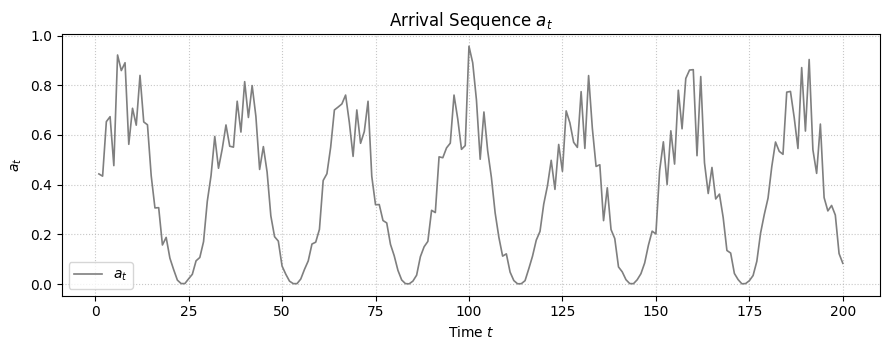
\includegraphics[width=0.8\linewidth]{control/arrival.png}
    \caption{Arrival process \(a_t\) for \(t \in [0, 200]\).}
    \label{fig:arrival-0-200}
\end{figure}

\medskip
The cost function at time \(t\) is choses as
\[
c_t(b, u)
=
\bigl(1 + \xi_t^b + \sin(2\pi t / P_b)\bigr)\,(1 - b)^2
\;+\;
\bigl(1 + \xi_t^u + \sin(2\pi t / P_u)\bigr)\,(1 - u)^2,
\]
where
\[
\xi_t^b,\, \xi_t^u \sim \mathrm{Uniform}(0, 0.5),
\qquad
P_b = 5, \quad P_u = 10.
\]
Here \(\xi_t^b\) and \(\xi_t^u\) represent independent random perturbations that model temporal variability in the state and control cost components.


We consider two simulation settings, with common parameters
\[
    T = 1000 \quad \text{(horizon length)}, \qquad
    H = 100 \quad \text{(feature dimension)},
\]
and vary the parameter \(\kappa \in \{0.1, 0.4\}.\)


We compare the following controllers:
\begin{itemize}
    \item \textbf{Offline optimal:} The best fixed weight vector \(w^*\), chosen in hindsight. 
    Note that the value of \(w^*\) depends on the choice of \(\kappa\).


    \item \textbf{Best linear controller:} \(u_t^K = K \cdot b_t\) with \(K = 0.53 \in [0,1]\). 
    This is the best controller within the class \(\{u_t^K : K \in [0,1]\}\), where the optimal
    value \(K = 0.53\) is obtained via numerical evaluation over a mesh.

    \item \textbf{Arbitrary linear controller:} \(u_t^K = K \cdot b_t\) with \(K = 0.2 \in [0,1]\).
    This serves as a simple baseline linear controller for comparison.

    \item \textbf{EGPC[\(\eta^*\)]:} The Exponentiated Gradient Perturbation Controller
    (Algorithm~\ref{alg:egpc}) with stepsize \(\eta^*\).

    \item \textbf{EGPC[\(\eta^{\mathrm{ind}}\)]:} The Exponentiated Gradient Perturbation Controller
    (Algorithm~\ref{alg:egpc}) with stepsize \(\eta^{\mathrm{ind}}\).
\end{itemize}









\subsection{Results}

Table~\ref{tab:kappa_results} reports the total cost of the different controllers for two
choices of the model parameter $\kappa \in \{0.1, 0.4\}$. In both cases, the linear
controllers serve as simple baselines, while the two variants of EGPC illustrate the
effect of using the theoretically optimal stepsize $\eta^\star$ versus the
$\kappa$-independent stepsize $\eta^{\mathrm{ind}}$.

\begin{table}[H]
\centering
\caption{Total cost comparison of different controllers for $\kappa = 0.4$ and $\kappa = 0.1$.}
\label{tab:kappa_results}
\begin{tabular}{lcc}
\hline
\textbf{Controller} 
    & $\boldsymbol{\kappa = 0.4}$ 
    & $\boldsymbol{\kappa = 0.1}$ \\
\hline
Offline optimal          
    & 963.8733 
    & 745.2144 \\[0.2em]
Linear $K = 0.53$        
    & 984.5877 
    & 984.5877 \\[0.2em]
Linear $K = 0.20$        
    & 2671.6528 
    & 2671.6528 \\[0.2em]
EGPC[$\eta^\star$]       
    & 1043.3331 \; ($\eta = 0.0034$) 
    & 2423.2565 \; ($\eta = 0.0009$) \\[0.2em]
EGPC[$\eta^{\mathrm{ind}}$] 
    & 1023.4862 \; ($\eta = 0.0089$) 
    & 973.2719 \; ($\eta = 0.0089$) \\
\hline
\end{tabular}
\end{table}

\subsection{Discussion: Trade-off in the choice of $\kappa$}

The parameter $\kappa$ controls the expressiveness of the comparator class: smaller
values of $\kappa$ correspond to a larger, more flexible policy class. This has two
opposing effects.

First, our theoretical regret bound scales as
\[
    \mathrm{Regret}(T) = O\!\left( \frac{\sqrt{T \log H}}{\kappa^4} \right)\quad  \text{ or }\quad O\!\left( \frac{\sqrt{T \log H}}{\kappa^2} \right),
\]
which \emph{increases} as $\kappa$ decreases. Thus, smaller $\kappa$ leads to a looser
regret guarantee and potentially larger deviation from the offline optimal policy.
This dependence is intuitively expected: a more expressive comparator class makes the
regret problem harder.

Second, the best offline policy $w^\star$ \emph{improves} as $\kappa$ decreases,
because the comparator class becomes richer. This can be seen in
Table~\ref{tab:kappa_results}, where the offline optimal cost for $\kappa = 0.1$ is
significantly smaller than for $\kappa = 0.4$.

However, the key quantity of interest in practice is not the regret itself but the
\emph{total cost achieved by the algorithm}. In this sense, the effect of $\kappa$ is
non-monotone. Although the offline optimal improves as $\kappa$ decreases, the regret
bound worsens, and therefore the algorithm's total performance does not necessarily
improve. Indeed, from Table~\ref{tab:kappa_results} we observe:

\begin{itemize}
    \item For the $\kappa$-independent stepsize $\eta^{\mathrm{ind}}$, moving from
    $\kappa = 0.1$ to $\kappa = 0.4$ slightly \emph{worsens} performance.
    \item For the theoretically optimal stepsize $\eta^\star$, performance
    \emph{improves} as $\kappa$ increases.
    \item Most importantly, the \textbf{gap between the offline optimal and EGPC
    shrinks as $\kappa$ increases}, which aligns with the theoretical regret bound.
\end{itemize}

Overall, neither the algorithm nor the theoretical analysis suggests an obvious
“best” choice of $\kappa$ for practical use. A smaller $\kappa$ enlarges the model
class and improves the offline benchmark but simultaneously makes regret minimization
harder. A larger $\kappa$ yields a smaller comparator class but leads to better regret
performance. The appropriate choice therefore depends on the desired balance between
model expressiveness and algorithmic stability.






\subsection{Simulation Figures}

In this section we present detailed simulation plots that illustrate the behavior of
the state dynamics, usage decisions, and incurred costs for both
$\kappa = 0.1$ and $\kappa = 0.4$.  
For each value of $\kappa$, we show:

\begin{itemize}
    \item State level trajectories.
    \item Instantaneous costs.
    \item Usage (allocation) decisions.
\end{itemize}

For our EGPC algorithm, we include several time-sliced views 
(e.g., $t \in [0,200]$, $[500,700]$, $[800,1000]$) to highlight the algorithm’s gradual 
convergence behavior.  
In contrast, the linear controller exhibits stationary behavior throughout the horizon
and therefore only requires a single short-horizon plot.

All offline-optimal curves correspond to the best fixed policy $w^\star$ for the 
specified value of $\kappa$.

\subsubsection{$\kappa = 0.1$ Results: State Level Trajectories}

\begin{figure}[H]
    \centering
    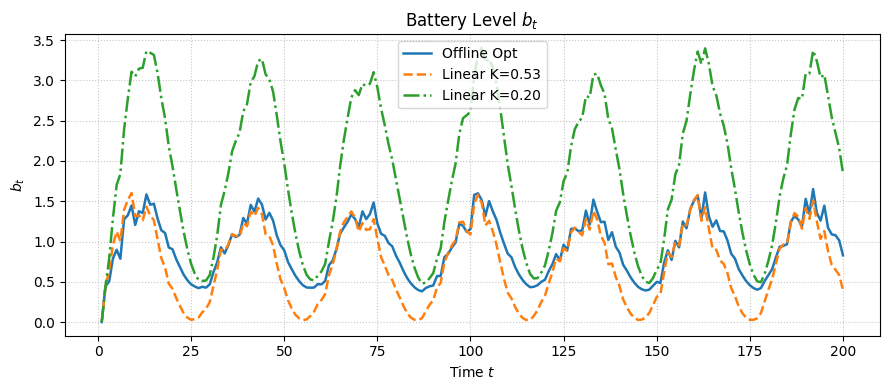
\includegraphics[width=0.8\textwidth]{control/kappa0.1/b-0-200-linears.png}
    \caption{State levels for the linear controllers ($K=0.53$ and $K=0.20$) versus
    the offline-optimal policy for $t \in [0,200]$, with $\kappa = 0.1$.
    The linear controllers produce repetitive, time-invariant behavior.}
\end{figure}

\begin{figure}[H]
    \centering
    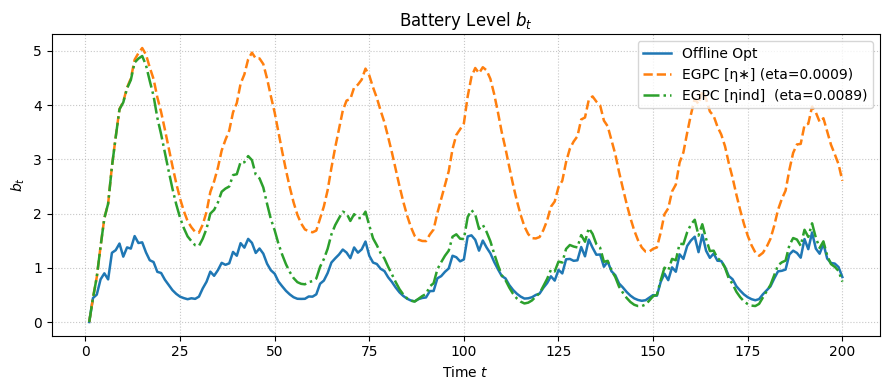
\includegraphics[width=0.8\textwidth]{control/kappa0.1/b-0-200-egpc.png}
    \caption{State levels for EGPC (two step sizes) versus the offline-optimal policy
    for $t \in [0,200]$, with $\kappa = 0.1$.
    This interval highlights the initial transient behavior before the controller stabilizes.}
\end{figure}

\begin{figure}[H]
    \centering
    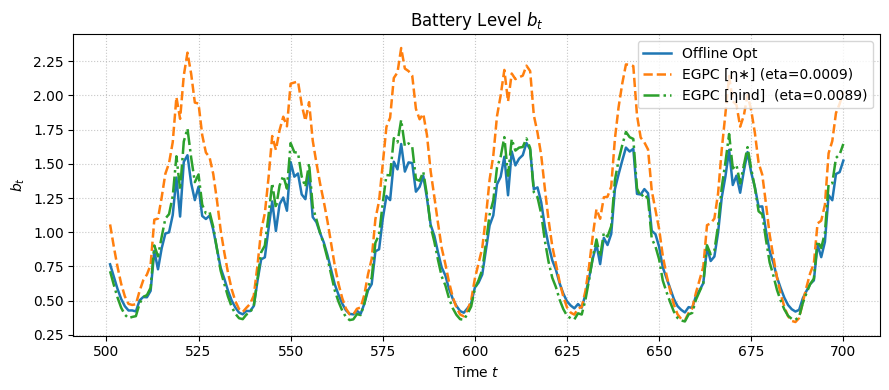
\includegraphics[width=0.8\textwidth]{control/kappa0.1/b-700-egpc.png}
    \caption{State levels for EGPC (two step sizes) versus the offline-optimal policy
    for $t \in [500,700]$, with $\kappa = 0.1$.
    This mid-horizon window illustrates the slow but consistent convergence trend.}
\end{figure}

\begin{figure}[H]
    \centering
    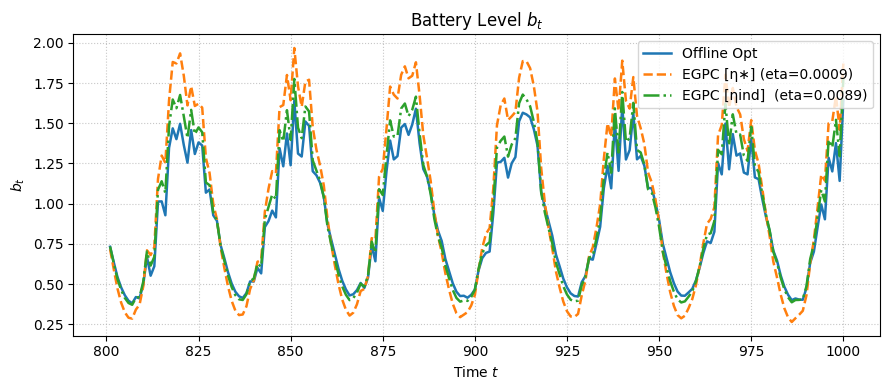
\includegraphics[width=0.8\textwidth]{control/kappa0.1/b-1000-egpc.png}
    \caption{State levels for EGPC (two step sizes) versus the offline-optimal policy
    for $t \in [800,1000]$, with $\kappa = 0.1$.
    By this stage, the controller has largely stabilized and the trajectories cluster tightly.}
\end{figure}



\subsubsection{$\kappa = 0.1$ Results: Instantaneous Costs}

\begin{figure}[H]
    \centering
    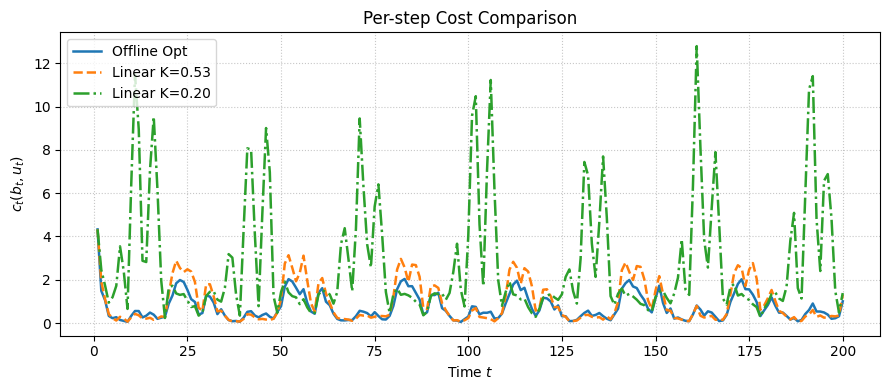
\includegraphics[width=0.8\textwidth]{control/kappa0.1/c-0-200-linears.png}
    \caption{Instantaneous costs for the linear controllers versus the offline-optimal policy
    for $t \in [0,200]$, with $\kappa = 0.1$.}
\end{figure}

\begin{figure}[H]
    \centering
    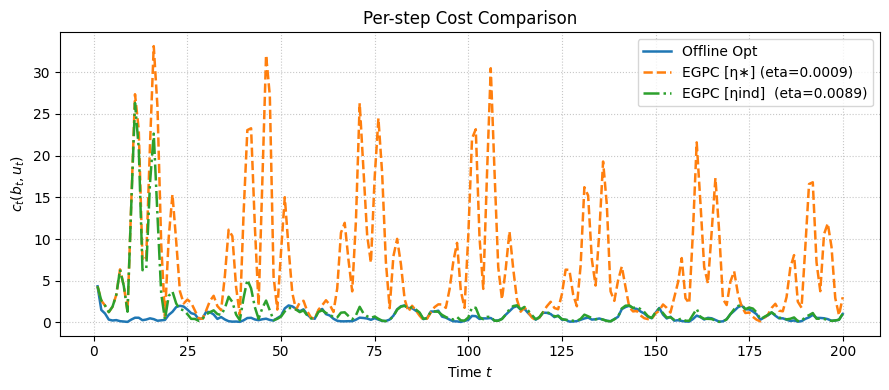
\includegraphics[width=0.8\textwidth]{control/kappa0.1/c-0-200-egpc.png}
    \caption{Instantaneous costs for EGPC (two step sizes) versus the offline-optimal policy
    for $t \in [0,200]$, with $\kappa = 0.1$.
    This interval shows the initial fluctuation in costs as the controller adapts.}
\end{figure}

\begin{figure}[H]
    \centering
    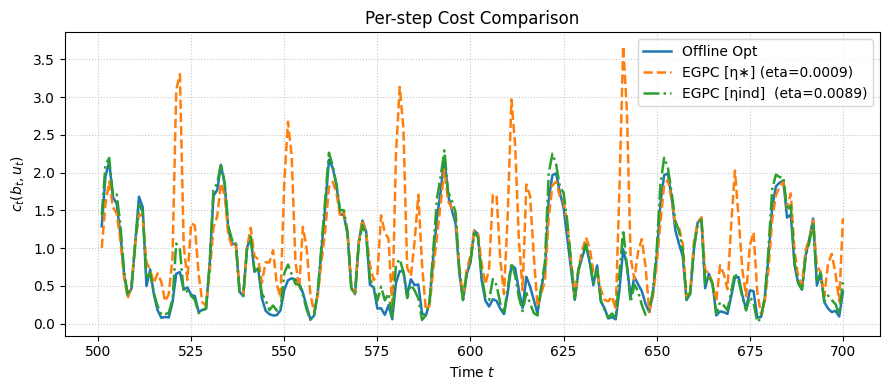
\includegraphics[width=0.8\textwidth]{control/kappa0.1/c-700-egpc.png}
    \caption{Instantaneous costs for EGPC (two step sizes) versus the offline-optimal policy
    for $t \in [500,700]$, with $\kappa = 0.1$.
    This figure demonstrates how the cost curves compress as the algorithm approaches
    stable behavior.}
\end{figure}

\begin{figure}[H]
    \centering
    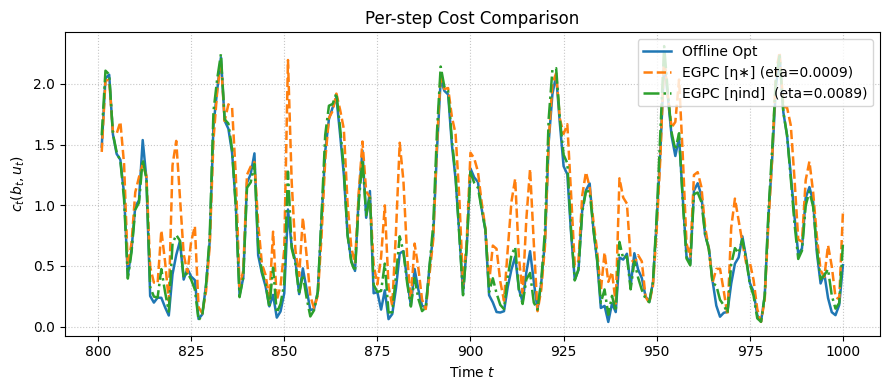
\includegraphics[width=0.8\textwidth]{control/kappa0.1/c-1000-egpc.png}
    \caption{Instantaneous costs for EGPC (two step sizes) versus the offline-optimal policy
    for $t \in [800,1000]$, with $\kappa = 0.1$.
    By the end of the horizon, the cost trajectories closely track the offline-optimal benchmark.}
\end{figure}



\subsubsection{$\kappa = 0.1$ Results: Usage (Allocation) Decisions}

\begin{figure}[H]
    \centering
    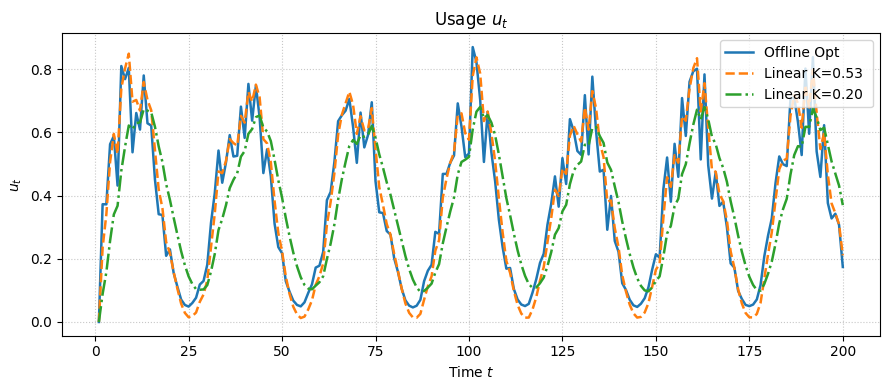
\includegraphics[width=0.8\textwidth]{control/kappa0.1/u-0-200-linears.png}
    \caption{Usage $u_t$ for the linear controllers versus the offline-optimal policy
    for $t \in [0,200]$, with $\kappa = 0.1$.}
\end{figure}

\begin{figure}[H]
    \centering
    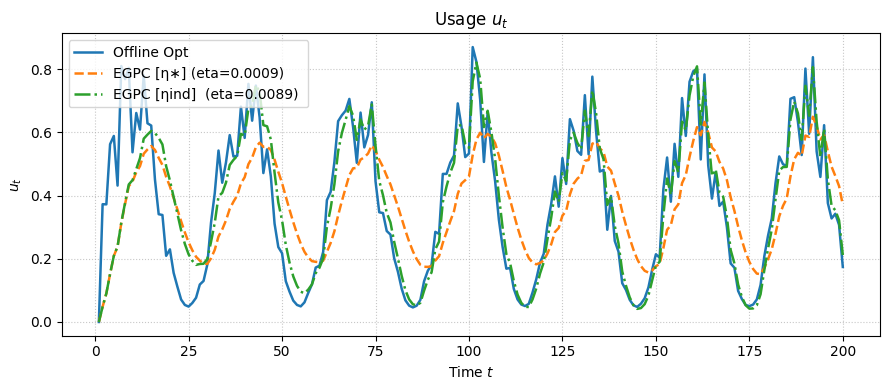
\includegraphics[width=0.8\textwidth]{control/kappa0.1/u-0-200-egpc.png}
    \caption{Usage $u_t$ for EGPC (two step sizes) versus the offline-optimal policy
    for $t \in [0,200]$, with $\kappa = 0.1$.
    This interval captures the initial adaptation of the usage decisions.}
\end{figure}

\begin{figure}[H]
    \centering
    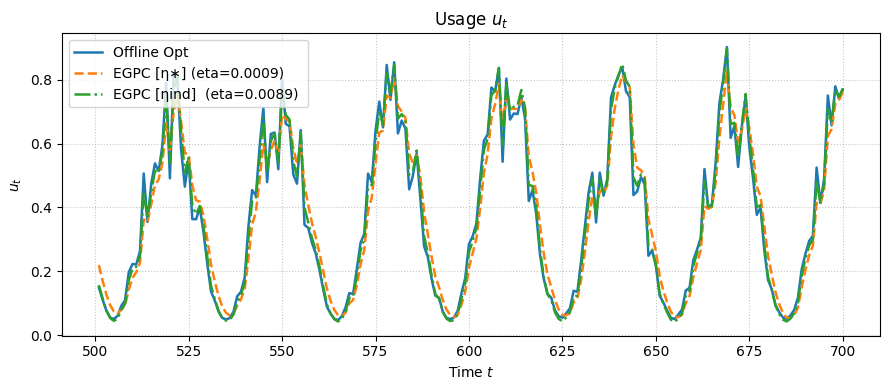
\includegraphics[width=0.8\textwidth]{control/kappa0.1/u-700-egpc.png}
    \caption{Usage $u_t$ for EGPC (two step sizes) versus the offline-optimal policy
    for $t \in [500,700]$, with $\kappa = 0.1$.
    The mid-horizon behavior shows reduced variability and improved alignment with the benchmark.}
\end{figure}

\begin{figure}[H]
    \centering
    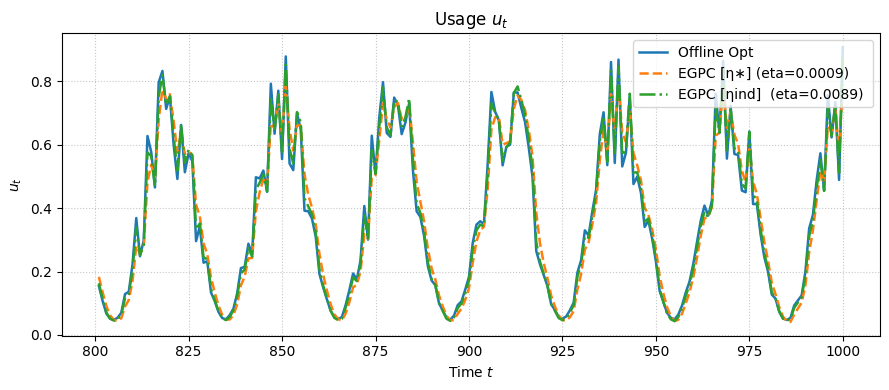
\includegraphics[width=0.8\textwidth]{control/kappa0.1/u-1000-egpc.png}
    \caption{Usage $u_t$ for EGPC (two step sizes) versus the offline-optimal policy
    for $t \in [800,1000]$, with $\kappa = 0.1$.
    This final segment shows the stabilization of usage decisions around the offline-optimal policy.}
\end{figure}



























\subsubsection{$\kappa = 0.4$ Results: State Level Trajectories}

\begin{figure}[H]
    \centering
    
\includegraphics[width=0.8\textwidth]{control/kappa0.4/b-0-200-linears.png}
    \caption{State levels for the linear controllers ($K=0.53$ and $K=0.20$) versus
    the offline-optimal policy for $t \in [0,200]$, with $\kappa = 0.4$.
    The linear controllers produce repetitive, time-invariant behavior.}
\end{figure}

\begin{figure}[H]
    \centering
    
\includegraphics[width=0.8\textwidth]{control/kappa0.4/b-0-200-egpc.png}
    \caption{State levels for EGPC (two step sizes) versus the offline-optimal policy
    for $t \in [0,200]$, with $\kappa = 0.4$.
    This interval highlights the initial transient behavior before the controller stabilizes.}
\end{figure}

\begin{figure}[H]
    \centering
    
\includegraphics[width=0.8\textwidth]{control/kappa0.4/b-700-egpc.png}
    \caption{State levels for EGPC (two step sizes) versus the offline-optimal policy
    for $t \in [500,700]$, with $\kappa = 0.4$.
    This mid-horizon window illustrates the slow but consistent convergence trend.}
\end{figure}

\begin{figure}[H]
    \centering
    
\includegraphics[width=0.8\textwidth]{control/kappa0.4/b-1000-egpc.png}
    \caption{State levels for EGPC (two step sizes) versus the offline-optimal policy
    for $t \in [800,1000]$, with $\kappa = 0.4$.
    By this stage, the controller has largely stabilized and the trajectories cluster tightly.}
\end{figure}



\subsubsection{$\kappa = 0.4$ Results: Instantaneous Costs}

\begin{figure}[H]
    \centering
    
\includegraphics[width=0.8\textwidth]{control/kappa0.4/c-0-200-linears.png}
    \caption{Instantaneous costs for the linear controllers versus the offline-optimal policy
    for $t \in [0,200]$, with $\kappa = 0.4$.}
\end{figure}

\begin{figure}[H]
    \centering
    
\includegraphics[width=0.8\textwidth]{control/kappa0.4/c-0-200-egpc.png}
    \caption{Instantaneous costs for EGPC (two step sizes) versus the offline-optimal policy
    for $t \in [0,200]$, with $\kappa = 0.4$.
    This interval shows the initial fluctuation in costs as the controller adapts.}
\end{figure}

\begin{figure}[H]
    \centering
    
\includegraphics[width=0.8\textwidth]{control/kappa0.4/c-700-egpc.png}
    \caption{Instantaneous costs for EGPC (two step sizes) versus the offline-optimal policy
    for $t \in [500,700]$, with $\kappa = 0.4$.
    This figure demonstrates how the cost curves compress as the algorithm approaches
    stable behavior.}
\end{figure}

\begin{figure}[H]
    \centering
    
\includegraphics[width=0.8\textwidth]{control/kappa0.4/c-1000-egpc.png}
    \caption{Instantaneous costs for EGPC (two step sizes) versus the offline-optimal policy
    for $t \in [800,1000]$, with $\kappa = 0.4$.
    By the end of the horizon, the cost trajectories closely track the offline-optimal benchmark.}
\end{figure}



\subsubsection{$\kappa = 0.4$ Results: Usage (Allocation) Decisions}

\begin{figure}[H]
    \centering
    
\includegraphics[width=0.8\textwidth]{control/kappa0.4/u-0-200-linears.png}
    \caption{Usage $u_t$ for the linear controllers versus the offline-optimal policy
    for $t \in [0,200]$, with $\kappa = 0.4$.}
\end{figure}

\begin{figure}[H]
    \centering
    
\includegraphics[width=0.8\textwidth]{control/kappa0.4/u-0-200-egpc.png}
    \caption{Usage $u_t$ for EGPC (two step sizes) versus the offline-optimal policy
    for $t \in [0,200]$, with $\kappa = 0.4$.
    This interval captures the initial adaptation of the usage decisions.}
\end{figure}

\begin{figure}[H]
    \centering
    
\includegraphics[width=0.8\textwidth]{control/kappa0.4/u-700-egpc.png}
    \caption{Usage $u_t$ for EGPC (two step sizes) versus the offline-optimal policy
    for $t \in [500,700]$, with $\kappa = 0.4$.
    The mid-horizon behavior shows reduced variability and improved alignment with the benchmark.}
\end{figure}

\begin{figure}[H]
    \centering
    
\includegraphics[width=0.8\textwidth]{control/kappa0.4/u-1000-egpc.png}
    \caption{Usage $u_t$ for EGPC (two step sizes) versus the offline-optimal policy
    for $t \in [800,1000]$, with $\kappa = 0.4$.
    This final segment shows the stabilization of usage decisions around the offline-optimal policy.}
\end{figure}










\section{Extension to the Multi-Sink Setting}

We extend the single-sink setting to a \emph{multi-sink} scenario, where at each round \(t\) the controller selects a vector
\[
x_t \in \mathbb{R}_{\ge 0}^n,
\]
whose \(i\)-th component \(x_t^{(i)}\) denotes the resource allocated to sink (task) \(i \in \{1,\ldots,n\}\).
The system then incurs a cost
\[
c_t(b_t, x_t),
\]
where \(c_t : [0,B] \times \mathbb{R}_{\ge 0}^n \to \mathbb{R}\) is convex in its arguments.  
We further assume that each \(c_t\) satisfies the following Lipschitz condition:
\begin{equation}
\label{eq:lip-c-x}
|c_t(b, x) - c_t(b', x')|
\;\le\;
L_b\, |b - b'| \;+\; L_x\, \|x - x'\|_1 .
\end{equation}

The total resource used in round \(t\) equals the \(\ell_1\)-norm of the allocation vector,
\[
u_t \;=\; \|x_t\|_1 \;=\; \sum_{i=1}^n x_t^{(i)},
\]
and the state evolves according to
\begin{equation}
\label{eq:battery-evo-W}
    b_{t+1} \;=\; \min\{\, B,\, b_t - u_t + a_t \,\}.
\end{equation}
All constraints remain expressed in terms of \(u_t\).

This formulation enables resources to be distributed among multiple tasks while preserving the linear state dynamics.
It introduces additional decision complexity but retains much of the analytical structure of the single-sink model.  





\subsection{Policy class}
% One possible class to consider is again the constrained \(\mathrm{DAC}\).  
% While this class offers high expressiveness and can model more complex scenarios, it suffers from the same computational inefficiency issues.


Here we introduce the direct generlizion of the vector $\mathrm{SDAC}$ policy class.
Fix design parameters \(\kappa \in [0,1]\) and a memory horizon \(H \in \mathbb{N}\).  For any matrix \(W\)  in the probability simplex
\[
\Delta_{n \times H} \;\coloneqq\;
\biggl\{\,W\in\mathbb{R}^{n\times H} \;\bigm|\; W^{(i,j)} \ge 0, \;\; \sum_{i=1}^n\sum_{j=1}^H W^{(i,j)} = 1 \,\biggr\},
\]
we define a policy \(\pi(W) \in \mathrm{S2DAC}_H^\kappa\) by
\begin{equation}\label{eq:x-of-efficient}
x_t^{i,\pi(W)} \;=\; \frac{\kappa}{n} b_t^{\pi(W)} \;+\; \sum_{j=1}^H W^{(i,j)} (1-\kappa)^j \, a_{t-j},
\end{equation}
with the convention \(a_\tau \equiv 0\) for \(\tau \le 0\).

Using the the same definition we put  weighted arrival history into the vector
\[
\vec{a}_t
\;\coloneqq\;
\bigl((1-\kappa)^1 a_{t-1},\; (1-\kappa)^2 a_{t-2},\;\dots,\; (1-\kappa)^H a_{t-H}\bigr)^\top
\in \mathbb{R}^H ,
\]
so that \eqref{eq:x-of-efficient} becomes
\begin{equation}
    \label{eq:x-vec-1}
    x_t^{\pi(W)} \;=\; \frac{\kappa}{n}\, b_t^{\pi(W)} \mathbf{1} \;+\; W \vec{a}_t
\end{equation}
Define the sum of the elements in column \(j\) of the matrix \(W\) by
\[
w^{(j)}
=
\sum_{i=1}^n W^{(i,j)},
\]
and collect these into the vector
\[
w = \big( w^{(1)}, w^{(2)}, \ldots, w^{(H)} \big)^\top \in \Delta_H.
\]
or equivalently
\[
w = 
W^\top \mathbf{1}
\]
Then we can write 
\[
u_t^{\pi(W)}
=
\sum_{i=1}^n x_t^{i,\pi(W)}
=
\kappa b_t^{\pi(W)}
+
\sum_{i=1}^n \sum_{j=1}^H  W(i,j) (1-\kappa)^j a_{t-j}
=
\kappa b_t^{\pi(W)}
+
\langle w,\vec{a}_t\rangle
\]





\begin{Thm:Lemma}\label{lem:w-l1-W}
For any integers \( t \) and \( i \) such that \( 1 \leq i \leq t \),
\[
\|w_{t-i} - w_t\|_1 \leq \|W_{t-i} - W_t\|_1.
\]
\end{Thm:Lemma}

\begin{proof}
By definition, each coordinate of \(w_t\) is given by
\[
w_t^{(j)} = \sum_{k=1}^n W_t^{(k,j)}.
\]
Hence,
\[
w_{t-i}^{(j)} - w_t^{(j)} = \sum_{k=1}^n \big( W_{t-i}^{(k,j)} - W_t^{(k,j)} \big).
\]
Taking the \(\ell_1\)-norm, we have
\begin{align*}
\|w_{t-i}-w_t\|_1
&= \sum_{j=1}^n \big| w_{t-i}^{(j)} - w_t^{(j)} \big| \\
&= \sum_{j=1}^n \left| \sum_{k=1}^n \big( W_{t-i}^{(k,j)} - W_t^{(k,j)} \big) \right| \\
&\leq \sum_{j=1}^n \sum_{k=1}^n \big| W_{t-i}^{(k,j)} - W_t^{(k,j)} \big| \\
&= \|W_{t-i} - W_t\|_1.
\end{align*}
\end{proof}



\begin{Thm:Remark}\label{rem:4-lem}
Lemmas \ref{lem:no-sat}, \ref{lem:state-decomp}, \ref{lem:prefix-linear}, and \ref{lem:feasible} apply directly to the analysis in this section and remain valid without modification.
\end{Thm:Remark}





\begin{Thm:Lemma}\label{lem:prefix-linear-x}
Fix \((\kappa, H)\) and a weight matrix \( W \in \Delta_{n \times H} \).  
Suppose the policy \( \pi(W) \in \mathrm{S2DAC}_H^\kappa \) is applied from \( t = 1 \) up to round \( t \).  
Then, the round-\(t\) allocation is a linear functional of \( W \):
\[
x_t^{\pi(W)} 
=
\frac{\kappa}{n} (\mathbf{1}\mathbf{1}^\top) W \psi_t 
\;+\;
W \vec{a}_t,
\]
or equivalently, for each component \( i \in [n] \),
\[
x_t^{i,\pi(W)} 
=
\frac{\kappa}{n}\,
\mathbf{1}^\top W \psi_t
+
\sum_{j=1}^H W^{(i,j)} (1-\kappa)^j a_{t-j}.
\]
\end{Thm:Lemma}

\begin{proof}
By Remark~\ref{rem:4-lem}, Lemma~\ref{lem:state-decomp} applies, implying that
\[
b_t^{\pi(W)}
= \langle w, \psi_t \rangle
= (W^\top \mathbf{1})^\top \psi_t
= \mathbf{1}^\top W \psi_t.
\]
Substituting this expression into \eqref{eq:x-vec-1}, we obtain
\[
x_t^{\pi(W)} 
= \frac{\kappa}{n} \mathbf{1} (\mathbf{1}^\top W \psi_t) + W \vec{a}_t
= \frac{\kappa}{n} (\mathbf{1}\mathbf{1}^\top) W \psi_t + W \vec{a}_t.
\]
Expanding by component and using the definition of \(\vec{a}_t\) from \eqref{eq:x-of-efficient} yields
\[
x_t^{i,\pi(W)}
= \frac{\kappa}{n} \mathbf{1}^\top W \psi_t
+ \sum_{j=1}^H W^{(i,j)} (1-\kappa)^j a_{t-j}.
\]
Thus, the mapping \( W \mapsto x_t^{\pi(W)} \) is linear, completing the proof.
\end{proof}


\begin{Thm:Lemma}[Convexity and Lipschitz continuity of the surrogate cost]
\label{lem:surrogate-props-W}
For any round \(t\), define
\[
\ell_t(W) \;\coloneqq\; 
c_t\!\bigl(b_t^{\pi(W)},\,x_t^{\pi(W)}\bigr), \qquad W\in\Delta_{n\times H}.
\]
Then:
\begin{enumerate}
    \item \textbf{Convexity.} \(\ell_t\) is convex in \(W\).
    \item \textbf{Lipschitz continuity.} For all \(W,W'\in\Delta_{n\times H}\),
    \[
    \bigl|\ell_t(W)-\ell_t(W')\bigr| \;\le\; L\,\|W-W'\|_1,
    \qquad\text{with}\qquad
    L \;\coloneqq\; \frac{L_b}{\kappa} \;+\; 2L_x.
    \]
\end{enumerate}
\end{Thm:Lemma}

\begin{proof}
\textbf{Convexity.}
By Remark~\ref{rem:4-lem}, Lemma~\ref{lem:state-decomp} gives
\[
b_t^{\pi(W)} \;=\; \langle w,\psi_t\rangle \;=\; \mathbf{1}^\top W \psi_t,
\]
and Lemma~\ref{lem:prefix-linear-x} yields
\[
x_t^{\pi(W)} 
\;=\;
\frac{\kappa}{n}\,(\mathbf{1}\mathbf{1}^\top)W\psi_t \;+\; W\vec{a}_t.
\]
Hence, both \(b_t^{\pi(W)}\) and \(x_t^{\pi(W)}\) are linear in \(W\). Since \(c_t(\cdot,\cdot)\) is convex and convexity is preserved under pre-composition with linear maps, \(\ell_t(W)=c_t\!\bigl(b_t^{\pi(W)},x_t^{\pi(W)}\bigr)\) is convex.

\medskip
\textbf{Lipschitz continuity.}
By the assumed coordinatewise Lipschitz property of \(c_t\) (cf. Eq.~\ref{eq:lip-c-x}),
\begin{equation}\label{eq:sur-lip-base}
\bigl|\ell_t(W)-\ell_t(W')\bigr|
\;\le\;
L_b\,\bigl|b_t^{\pi(W)}-b_t^{\pi(W')}\bigr|
\;+\;
L_x\,\bigl\|x_t^{\pi(W)}-x_t^{\pi(W')}\bigr\|_1.
\end{equation}
For the first term, using \(b_t^{\pi(W)}=\mathbf{1}^\top W\psi_t\),
\[
\bigl|b_t^{\pi(W)}-b_t^{\pi(W')}\bigr|
=
\bigl|\mathbf{1}^\top (W-W')\psi_t\bigr|
=
\bigl|\langle (W-W')^\top\mathbf{1},\,\psi_t\rangle\bigr|
\;\le\;
\|(W-W')^\top\mathbf{1}\|_1\,\|\psi_t\|_\infty.
\]
By Lemma~\ref{lem:w-l1-W}, \(\|(W-W')^\top\mathbf{1}\|_1\le \|W-W'\|_1\). Using the bound \(\|\psi_t\|_\infty\le 1/\kappa\) (from Lemma~\ref{lem:state-decomp}),
\begin{equation}\label{eq:b-lip}
\bigl|b_t^{\pi(W)}-b_t^{\pi(W')}\bigr|
\;\le\;
\frac{1}{\kappa}\,\|W-W'\|_1.
\end{equation}

For the second term, using \(x_t^{\pi(W)}=\frac{\kappa}{n}\mathbf{1}\bigl(\mathbf{1}^\top W\psi_t\bigr)+W\vec{a}_t\) (Eq.~\ref{eq:x-vec-1}),
\begin{align*}
\bigl\|x_t^{\pi(W)}-x_t^{\pi(W')}\bigr\|_1
&=
\left\|\frac{\kappa}{n}\,\mathbf{1}\,\bigl(\mathbf{1}^\top (W-W')\psi_t\bigr)
\;+\;
(W-W')\vec{a}_t\right\|_1 \\
&\le
\frac{\kappa}{n}\,\|\mathbf{1}\|_1\,\bigl|\mathbf{1}^\top (W-W')\psi_t\bigr|
\;+\;
\|(W-W')\vec{a}_t\|_1 \\
&=
\kappa\,\bigl|b_t^{\pi(W)}-b_t^{\pi(W')}\bigr|
\;+\;
\|W-W'\|_1\,\|\vec{a}_t\|_\infty.
\end{align*}
By assumption \(\|\vec{a}_t\|_\infty\le 1\), and combining with \eqref{eq:b-lip},
\begin{equation}\label{eq:x-lip}
\bigl\|x_t^{\pi(W)}-x_t^{\pi(W')}\bigr\|_1
\;\le\;
\kappa\cdot \frac{1}{\kappa}\,\|W-W'\|_1 \;+\; \|W-W'\|_1
\;=\;
2\,\|W-W'\|_1.
\end{equation}

Finally, substituting \eqref{eq:b-lip} and \eqref{eq:x-lip} into \eqref{eq:sur-lip-base} gives
\[
\bigl|\ell_t(W)-\ell_t(W')\bigr|
\;\le\;
\left(\frac{L_b}{\kappa}+2L_x\right)\,\|W-W'\|_1,
\]
which establishes the claimed Lipschitz constant \(L=L_b/\kappa+2L_x\).
\end{proof}









\subsection{Algorithm}

We now present the generalized version of Algorithm~\ref{alg:egpc} for the multi-allocation setting.  
The full procedure, termed the \emph{Multi-Exponentiated-Gradient Perturbation Controller (MEGPC)}, is outlined below.

\begin{algorithm}
\caption{Multi-Exponentiated-Gradient Perturbation Controller (MEGPC)}
\label{alg:megpc}
\begin{algorithmic}[1]
\Require Horizon \(T\), step size \(\eta > 0\), initialization \(W_1 \in \Delta_{n\times H}\), and \(b_1 = 0\).

\For{$t = 1$ to $T$}

    \State 
    \(
        \widehat{x}_t^{\mathcal{A}} 
        \gets
        \frac{\kappa}{n}\, b_t^{\mathcal{A}}\, \mathbf{1}
        +
        W_t \vec{a}_t
    \)
    \State
    \(
        \widehat{u}_t^{\mathcal{A}} 
        \gets
        \|\widehat{x}_t^{\mathcal{A}}\|_1
        =
        \kappa b_t^{\mathcal{A}} + \langle w_t , \vec{a}_t\rangle
    \)

    \State \textbf{Apply feasible allocation:}
    \[
        u_t^{\mathcal{A}} \gets \min\{\widehat{u}_t^{\mathcal{A}},\, b_t^{\mathcal{A}}\},
        \qquad
        x_t^{\mathcal{A}} \gets
        \widehat{x}_t^{\mathcal{A}} \cdot
        \frac{u_t^{\mathcal{A}}}{\widehat{u}_t^{\mathcal{A}}}
    \]

    \State \textbf{Update internal state:}
    \[
        b_{t+1}^{\mathcal{A}} \gets b_t^{\mathcal{A}} + a_t - u_t^{\mathcal{A}}
    \]

    \State \textbf{Construct and evaluate surrogate cost:}
    \[
        \ell_t(W)
        \coloneqq
        c_t\!\bigl(b_t^{\pi(W)},\,x_t^{\pi(W)}\bigr)
    \]

    \State \textbf{Exponentiated-Gradient update over the simplex:}
    \For{each $(i,j) \in \{1,\dots,n\} \times \{1,\dots,H\}$}
        \[
            \widehat{W}_{t+1}^{(i,j)} 
            \gets
            W_t^{(i,j)} 
            \exp\!\big(-\eta\, (\nabla \ell_t(W_t))^{(i,j)}\big)
        \]
    \EndFor
    \[
        W_{t+1}^{(i,j)} 
        \gets
        \frac{\widehat{W}_{t+1}^{(i,j)}}
        {\sum_{i'=1}^n \sum_{j'=1}^H \widehat{W}_{t+1}^{(i',j')}}.
    \]
\EndFor
\end{algorithmic}
\end{algorithm}

\subsection{Regret Analysis}

We decompose the regret of our controller relative to the comparator class \(\mathrm{S2DAC}_H^\kappa\).  
For horizon \(T\),
\begin{align*}
\sum_{t=1}^T c_t(b_t^\mathcal{A},x_t^\mathcal{A})
- \min_{\pi\in\mathrm{S2DAC}_H^\kappa} \sum_{t=1}^T c_t(b_t^\pi,x_t^\pi)
&=
\underbrace{\sum_{t=1}^T \big[ c_t(b_t^\mathcal{A},x_t^\mathcal{A}) - c_t(b_t^{\pi(W_t)},x_t^{\pi(W_t)}) \big]}_{\text{Approximation gap}} \\
&\quad+\;
\underbrace{\sum_{t=1}^T \big[ c_t(b_t^{\pi(W_t)},x_t^{\pi(W_t)}) - c_t(b_t^{\pi(W^*)},x_t^{\pi(W^*)}) \big]}_{\text{Learning regret}},
\end{align*}
where
\[
W^* \in \arg\min_{W\in\Delta_H} \sum_{t=1}^T c_t(b_t^{\pi(W)},x_t^{\pi(W)}).
\]

The \textit{learning regret} is controlled via standard Online Mirror Descent bounds, while the \textit{approximation gap} measures the deviation between the controller’s realized and surrogate actions under the same weight sequence.

\subsubsection{Bounding the Learning Regret}

We bound the learning regret using standard Online Mirror Descent (OMD) results.  
With the negative-entropy regularizer
\[
\Psi(W) = \sum_{i=1}^H \sum_{j=1}^n W^{(i,j)} \log W^{(i,j)},
\]
Algorithm~\ref{alg:megpc} corresponds to OMD with this mirror map. By the standard OMD guarantee (see, e.g., \cite{orabona_modern_2023}),
\[
\sum_{t=1}^T 
\left\langle g_t,\, W_t - W^* \right\rangle
\le
\frac{\log(nH)}{\eta}
+ \frac{\eta}{2}\sum_{t=1}^T \|g_t\|_\infty^2,
\]
where \(g_t \in \partial \ell_t(W_t)\).

From Lemma~\ref{lem:surrogate-props-W}, each \(\ell_t\) is convex and \(L\)-Lipschitz under the \(\ell_1\)-norm, implying \(\|g_t\|_\infty \le L\).  
Hence,
\[
\sum_{t=1}^T \bigl(\ell_t(W_t) - \ell_t(W^*)\bigr)
\le
\frac{\log(nH)}{\eta}
+ \frac{\eta L^2 T}{2}.
\]
Therefore, the learning regret satisfies
\begin{equation}
\label{eq:omd-W}
\sum_{t=1}^T 
\Big(
c_t(b_t^{\pi(W_t)},x_t^{\pi(W_t)})
-
c_t(b_t^{\pi(W^*)},x_t^{\pi(W^*)})
\Big)
\le
\frac{\log(nH)}{\eta}
+ \frac{\eta L^2 T}{2}.
\end{equation}

\subsubsection{Bounding the OMD Step: Movement of the Weights}

We now bound the per-round variation of the simplex weights produced by the entropic OMD update.  
Using the same reasoning as in Corollary~\ref{cor:cum-move}, we obtain the following result.

\begin{Thm:Corollary}\label{cor:cum-move-W}
For the sequence of updates \(\{W_t\}_{t=1}^T\) generated by Algorithm~\ref{alg:megpc},  
the cumulative movement of the weights satisfies
\[
\|W_{t-i} - W_t\|_1
\;\le\;
\sum_{j=1}^i \|W_{t-j} - W_{t-j+1}\|_1
\;\le\;
i\,\eta L,
\]
where \(L\) is the Lipschitz constant of the surrogate costs \(\ell_t\) (from Lemma~\ref{lem:surrogate-props-W}).  
\end{Thm:Corollary}

\subsubsection{Bounding the Approximation Gap}

Define the state deviation as
\[
\Gamma_t^{W} \;\triangleq\; b_t^{\pi(W)} - b_t^{\mathcal{A}}.
\]

\begin{Thm:Remark}
The results of Lemmas~\ref{lem:bounding-u-eff} and~\ref{lem:state-gap-recursion-eff} extend directly to the multi-allocation case without modification.  
For all \(t\), the bounds on the effective usage hold as:
\begin{align}
\label{eq:u-lower-bound-eff-W}
u_t^{\mathcal{A}}
&\ge
\kappa\, b_t^{\mathcal{A}} + \langle w_t, \vec{a}_t \rangle
- (1-\kappa)\,[\Gamma_t^{W_t}]_+, \\[4pt]
\label{eq:u-upper-bound-eff-W}
u_t^{\mathcal{A}}
&\le
\kappa\, b_t^{\mathcal{A}} + \langle w_t, \vec{a}_t \rangle.
\end{align}

Similarly, the state recursion inequalities become:
\begin{align}
\label{eq:GAMMA-Lower-W}
\Gamma_{t+1}^{W}
&\ge
(1-\kappa)\,\Gamma_t^{W}
+ \langle w_t - w, \vec{a}_t \rangle
- (1-\kappa)\,[\Gamma_t^{W_t}]_+, \\[4pt]
\label{eq:GAMMA-Upper-W}
\Gamma_{t+1}^{W}
&\le
(1-\kappa)\,\Gamma_t^{W}
+ \langle w_t - w, \vec{a}_t \rangle.
\end{align}

\end{Thm:Remark}







\begin{Thm:Lemma}[State deviation bound]
\label{lem:state-gap-bound-W}
For all \(t\),
\[
-\frac{\eta L}{\kappa^3}
\;\leq\;
b_t^{\pi(W)} - b_t^\mathcal{A}
\;\leq\;
\frac{\eta L}{\kappa^2}.
\]
\end{Thm:Lemma}

\begin{proof}
\textbf{Upper bound.}  
From \eqref{eq:GAMMA-Upper-W},
\[
\Gamma_t^{W}
\;\leq\;
\sum_{i=1}^{t-1} (1-\kappa)^{i-1}\,\langle w_{t-i}-w,\,a_{t-i}\rangle .
\]
In particular, taking \(w=w_t\),
\[
\Gamma_t^{W_t}
\;\leq\;
\sum_{i=1}^{t-1} (1-\kappa)^{i-1}\,\langle w_{t-i}-w_t,\,a_{t-i}\rangle .
\]
Applying Hölder’s inequality and using \(a_{t-i}\in[0,1]\),
\[
\Gamma_t^{W_t}
\;\leq\;
\sum_{i=1}^{t-1} (1-\kappa)^{i-1}\,\|w_{t-i}-w_t\|_1 .
\]
Using Corollary~\ref{cor:cum-move-W} and Lemma~\ref{lem:w-l1-W} we get
\[
\Gamma_t^{W_t}
\;\leq\;
\eta L \sum_{i=1}^{t-1} i (1-\kappa)^{i-1}.
\]
Extending the sum to infinity and using \(\sum_{i=1}^\infty i (1-\kappa)^{i-1} = 1/\kappa^2\),
\begin{equation}
\label{eq:upper-gamma-final-W}
\Gamma_t^{W_t}
\;\leq\;
\frac{\eta L}{\kappa^2}.
\end{equation}

\medskip
\noindent
\textbf{Lower bound.}  
From \eqref{eq:GAMMA-Lower-W},
\[
\Gamma_t^W
\;\geq\;
\sum_{i=1}^{t-1} (1-\kappa)^{i-1}\,\langle w_{t-i}-w,\,a_{t-i}\rangle
-\sum_{i=1}^{t-1} (1-\kappa)^i\,[\Gamma_{t-i}^{W_{t-i}}]_+ .
\]
Choosing \(W=W_t\) and bounding the first term by \(-\|w_{t-i}-w_t\|_1\),
\[
\Gamma_t^{W_t}
\;\geq\;
-\sum_{i=1}^{t-1} (1-\kappa)^{i-1}\,\|w_{t-i}-w_t\|_1
-\frac{\eta L}{\kappa^2}\sum_{i=1}^{t-1} (1-\kappa)^i ,
\]
where the second sum uses the upper bound \eqref{eq:upper-gamma-final-W}.  
Applying Corollary~\ref{cor:cum-move-W} and Lemma~\ref{lem:w-l1-W},
\[
\Gamma_t^{W_t}
\;\geq\;
-\eta L \sum_{i=1}^{t-1} i (1-\kappa)^{i-1}
-\frac{\eta L}{\kappa^2}\sum_{i=1}^{t-1}(1-\kappa)^i .
\]
Extending both sums to infinity and evaluating,
\[
\sum_{i=1}^\infty i (1-\kappa)^{i-1} = \frac{1}{\kappa^2}, 
\qquad
\sum_{i=1}^\infty (1-\kappa)^i = \frac{1-\kappa}{\kappa},
\]
we obtain
\[
\Gamma_t^{W_t}
\;\geq\;
-\frac{\eta L}{\kappa^2} - \frac{\eta L(1-\kappa)}{\kappa^3}
\;\geq\;
-\frac{\eta L}{\kappa^3}.
\]

\medskip
\noindent
Combining the two bounds yields the claim.
\end{proof}






% \begin{Thm:Lemma}
% \label{lem:u-gap-by-b-gap-eff-W}
% For all \(t\),
% \[
% -\frac{\eta L}{\kappa^2}
% \;\leq\;
% \kappa \Gamma_t^{W_t}
% \;\leq\;
% u_t^{\pi(W_t)} - u_t^\mathcal{A}
% \;\leq\;
% \kappa \Gamma_t^{W_t}
% +(1-\kappa)\,[\Gamma_t^{W_t}]_+
% \;\leq\;
% \frac{\eta L}{\kappa^2}.
% \]
% \end{Thm:Lemma}

% \begin{proof}
% \textbf{Upper bound.}  
% From \eqref{eq:u-lower-bound-eff-W},
% \[
% u_t^\mathcal{A}
% \;\ge\;
% \kappa b_t^\mathcal{A} + \langle w_t,\vec{a}_t\rangle
% -(1-\kappa)\,[b_t^{\pi(W_t)}-b_t^\mathcal{A}]_+ .
% \]
% Subtracting from \(u_t^{\pi(W_t)} = \kappa b_t^{\pi(W_t)} + \langle W_t,\vec{a}_t\rangle\),
% \[
% u_t^{\pi(W_t)} - u_t^\mathcal{A}
% \;\le\;
% \kappa (b_t^{\pi(W_t)}-b_t^\mathcal{A})
% +(1-\kappa)\,[b_t^{\pi(W_t)}-b_t^\mathcal{A}]_+
% = \kappa \Gamma_t^{W_t} + (1-\kappa)\,[\Gamma_t^{W_t}]_+ .
% \]

% \textbf{Lower bound.}  
% From \eqref{eq:u-upper-bound-eff-W},
% \[
% u_t^\mathcal{A}
% \;\le\;
% \kappa b_t^\mathcal{A} + \langle w_t,\vec{a}_t\rangle ,
% \]
% so
% \[
% u_t^\mathcal{A} - u_t^{\pi(W_t)}
% \;\le\;
% \kappa b_t^\mathcal{A} + \langle w_t,\vec{a}_t\rangle
% - (\kappa b_t^{\pi(W_t)} + \langle w_t,\vec{a}_t\rangle)
% = -\kappa\Gamma_t^{W_t}.
% \]
% Equivalently,
% \[
% u_t^{\pi(W_t)} - u_t^\mathcal{A}
% \;\ge\; \kappa \Gamma_t^{W_t}.
% \]


% Substituting Lemma~\ref{lem:state-gap-bound-W} into the inequalities above completes the proof.
% \end{proof}




% \begin{Thm:Lemma}
%     \[
%     \|x_t^\mathcal{A} - x_t^{\pi(W_t)}\|_1
%     \leq     
%     2\frac{\eta L}{\kappa^2}
%     \]
% \end{Thm:Lemma}
% \begin{proof}
% \begin{align*}
%     \|x_t^\mathcal{A} - x_t^{\pi(W_t)}\|_1
%     &=
%     \|x_t^\mathcal{A} - \widehat{x}_t^\mathcal{A} +\widehat{x}_t^\mathcal{A} -x_t^{\pi(W_t)}\|_1
%     \\&\leq
%     \|x_t^\mathcal{A} - \widehat{x}_t^\mathcal{A}\|_1 + \|\widehat{x}_t^\mathcal{A} -x_t^{\pi(W_t)}\|_1
% \end{align*}    

% \begin{align*}
%     \|\widehat{x}_t^\mathcal{A} -x_t^{\pi(W_t)}\|_1
%     &=
%     \kappa |b_t^\mathcal{A}
%     - b_t^{\pi(W_t)}|
% \end{align*}

% For the other part we have:
% \begin{align*}
%     \|x_t^\mathcal{A} - \widehat{x}_t^\mathcal{A}\|_1
%     &=
%     \left\|\widehat{x}_t^\mathcal{A} \min\left(1,\frac{b_t^\mathcal{A}}{\|\widehat{x}_t^\mathcal{A}\|_1}\right) - \widehat{x}_t^\mathcal{A}\right\|_1
%     \\&=
%     \left\| \min\left({\|\widehat{x}_t^\mathcal{A}\|_1},{b_t^\mathcal{A}}\right) - {\|\widehat{x}_t^\mathcal{A}\|_1} \right\|_1
%     \\&=
%     \left\| \min\left(0,{b_t^\mathcal{A}} - {\|\widehat{x}_t^\mathcal{A}\|_1}\right) \right\|_1
%     \\&=
%     \left[\|\widehat{x}_t^\mathcal{A}\|_1 - b_t^\mathcal{A}\right]_+
%     \\&=
%     \left[\widehat{u}_t^\mathcal{A}- b_t^\mathcal{A}\right]_+
% \end{align*}
% By Algorithm~\ref{alg:megpc} we have
% \begin{align*}
%     \left[\widehat{u}_t^\mathcal{A}- b_t^\mathcal{A}\right]_+
%     =
%     \left[\langle w_t , \vec{a}_t\rangle - (1-\kappa) b_t^\mathcal{A}
%     \right]_+
%     \leq
%     (1-\kappa)\left[b_t^{\pi(W_t)} - b_t^\mathcal{A}
%     \right]_+
% \end{align*}
% where we used 
% \(u_t^{\pi(W_t)} \;=\; \kappa b_t^{\pi(W_t)} + \langle w_t,\vec{a}_t\rangle \;\le\; b_t^{\pi(W_t)},\)

% combinig these two  and using Lemma~\ref{lem:state-gap-bound-W} gives
% \begin{align*}
%     \|x_t^\mathcal{A} - x_t^{\pi(W_t)}\|_1
%     &\leq
%     (1-\kappa)\left[b_t^{\pi(W_t)} - b_t^\mathcal{A}
%     \right]_+
%     +
%     \kappa |b_t^\mathcal{A}
%     - b_t^{\pi(W_t)}|
%     \\&=
%     (1-\kappa)\left[b_t^{\pi(W_t)} - b_t^\mathcal{A}
%     \right]_+
%     +
%     \kappa \left[b_t^{\pi(W_t)} - b_t^\mathcal{A}
%     \right]_+
%     +
%     \kappa \left[b_t^\mathcal{A} -b_t^{\pi(W_t)}
%     \right]_+
%     \\&\leq
%     2\frac{\eta L}{\kappa^2}
% \end{align*}

% \end{proof}

\begin{Thm:Lemma}
\label{lem:x-gap-bound}
For all \(t\),
\[
\|x_t^{\mathcal{A}} - x_t^{\pi(W_t)}\|_1
\;\le\;
2\,\frac{\eta L}{\kappa^2}.
\]
\end{Thm:Lemma}

\begin{proof}
We decompose the difference as
\begin{align*}
\|x_t^{\mathcal{A}} - x_t^{\pi(W_t)}\|_1
&=
\|x_t^{\mathcal{A}} - \widehat{x}_t^{\mathcal{A}} + \widehat{x}_t^{\mathcal{A}} - x_t^{\pi(W_t)}\|_1
\\&\le
\|x_t^{\mathcal{A}} - \widehat{x}_t^{\mathcal{A}}\|_1
+ \|\widehat{x}_t^{\mathcal{A}} - x_t^{\pi(W_t)}\|_1.
\end{align*}

\textbf{Bounding the second term.}
By the definition of \(\widehat{x}_t^{\mathcal{A}}\) and \(x_t^{\pi(W_t)}\),
\[
\|\widehat{x}_t^{\mathcal{A}} - x_t^{\pi(W_t)}\|_1
=
\kappa\,|b_t^{\mathcal{A}} - b_t^{\pi(W_t)}|.
\]

\textbf{Bounding the first term.}
From Algorithm~\ref{alg:megpc},
\begin{align*}
\|x_t^{\mathcal{A}} - \widehat{x}_t^{\mathcal{A}}\|_1
&=
\left\|
\widehat{x}_t^{\mathcal{A}}
\!\left(
\min\!\left(1,\frac{b_t^{\mathcal{A}}}{\|\widehat{x}_t^{\mathcal{A}}\|_1}\right)
- 1
\right)
\right\|_1
\\&=
\left[\|\widehat{x}_t^{\mathcal{A}}\|_1 - b_t^{\mathcal{A}}\right]_+
=
[\widehat{u}_t^{\mathcal{A}} - b_t^{\mathcal{A}}]_+.
\end{align*}
By Algorithm~\ref{alg:megpc} and the definition of \(\widehat{u}_t^{\mathcal{A}}\),
\[
[\widehat{u}_t^{\mathcal{A}} - b_t^{\mathcal{A}}]_+
=
[\langle w_t, \vec{a}_t \rangle - (1-\kappa)b_t^{\mathcal{A}}]_+
\le
(1-\kappa)\,[b_t^{\pi(W_t)} - b_t^{\mathcal{A}}]_+,
\]
since \(u_t^{\pi(W_t)} = \kappa b_t^{\pi(W_t)} + \langle w_t, \vec{a}_t \rangle \le b_t^{\pi(W_t)}.\)

\textbf{Combining both parts.}
\begin{align*}
\|x_t^{\mathcal{A}} - x_t^{\pi(W_t)}\|_1
&\le
(1-\kappa)\,[b_t^{\pi(W_t)} - b_t^{\mathcal{A}}]_+
+ \kappa\,|b_t^{\mathcal{A}} - b_t^{\pi(W_t)}|
\\&=
(1-\kappa)\,[b_t^{\pi(W_t)} - b_t^{\mathcal{A}}]_+
+ \kappa\,[b_t^{\pi(W_t)} - b_t^{\mathcal{A}}]_+
+ \kappa\,[b_t^{\mathcal{A}} - b_t^{\pi(W_t)}]_+.
\end{align*}
Using Lemma~\ref{lem:state-gap-bound-W},
we obtain
\[
\|x_t^{\mathcal{A}} - x_t^{\pi(W_t)}\|_1
\le
2\,\frac{\eta L}{\kappa^2}.
\]
\end{proof}






\begin{Thm:Lemma}
\label{lem:stab-sum-W}
For all horizons \(T\),
\[
\sum_{t=1}^T \Big(
c_t\!\left(b_t^\mathcal{A},x_t^\mathcal{A}\right)
-
c_t\!\left(b_t^{\pi(W_t)},x_t^{\pi(W_t)}\right)
\Big)
\;\le\;
\frac{T \eta L^2}{\kappa^2},
\]
where \(L = 2 L_x + \tfrac{L_b}{\kappa}\).
\end{Thm:Lemma}
\begin{proof}
By Lipschitz continuity of \(c_t\) (Eq.~\eqref{eq:lip-c-x}),
\[
c_t\!\left(b_t^\mathcal{A},x_t^\mathcal{A}\right)
-
c_t\!\left(b_t^{\pi(W_t)},x_t^{\pi(W_t)}\right) 
\le
L_x \big\|x_t^\mathcal{A} - x_t^{\pi(W_t)}\big\|_1
+ L_b \big|b_t^\mathcal{A} - b_t^{\pi(W_t)}\big|.
\]
From Lemma~\ref{lem:x-gap-bound},
\[
|x_t^\mathcal{A} - x_t^{\pi(W_t)}|
\;\le\; 2\frac{\eta L}{\kappa^2},
\]
and from Lemma~\ref{lem:state-gap-bound-W}
\[
|b_t^\mathcal{A} - b_t^{\pi(W_t)}|
\;\le\; \frac{\eta L}{\kappa^3}.
\]
Therefore, for each \(t \ge 2\),
\[
c_t\!\left(b_t^\mathcal{A},x_t^\mathcal{A}\right)
-
c_t\!\left(b_t^{\pi(W_t)},x_t^{\pi(W_t)}\right)
\;\le\;
2L_x \frac{\eta L}{\kappa^2}
+ L_b \frac{\eta L}{\kappa^3}.
\]
Summing over \(t=1,2,\dots,T\) gives
\[
\sum_{t=2}^T
\Big(
c_t(b_t^\mathcal{A},x_t^\mathcal{A})
-
c_t(b_t^{\pi(W_t)},x_t^{\pi(W_t)})
\Big)
\;\le\;
(T-1)\frac{\eta L}{\kappa^2}\left(
2 L_x 
+  \frac{L_b}{\kappa}
\right).
\]
Since 
\(c_1(b_1^\mathcal{A},x_1^\mathcal{A})
=
c_1(b_1^{\pi(W_1)},x_1^{\pi(W_1)})\) and \(L = 2 L_x + \tfrac{L_b}{\kappa}\), this simplifies to
\[
\sum_{t=1}^T
\Big(
c_t(b_t^\mathcal{A},x_t^\mathcal{A})
-
c_t(b_t^{\pi(W_t)},x_t^{\pi(W_t)})
\Big)
\;\le\;
\frac{T \eta L^2}{\kappa^2}.
\]
\end{proof}


\subsubsection{Putting It Together}

\begin{Thm:Theorem}[Regret bound]
\label{thm:regret-W}
Suppose the costs \(c_t\) are convex and \(L\)-Lipschitz (with \(L = 2 L_x + \tfrac{L_b}{\kappa}\)).  
Then Algorithm~\ref{alg:megpc} with step size \(\eta>0\) satisfies
\[
\mathrm{Regret}(T)
\;\triangleq\;
\sum_{t=1}^T c_t(b_t^\mathcal{A},x_t^\mathcal{A})
\;-\;
\min_{W\in\Delta_{n\times H}}\sum_{t=1}^T c_t\!\big(b_t^{\pi(W)},x_t^{\pi(W)}\big)
\;\le\;
\frac{\log (nH)}{\eta} \;+\; \eta L^2 T\Big(\tfrac{1}{2} + \tfrac{1}{\kappa^2}\Big).
\]
With the optimal step size
\[
\eta^* \;=\; \sqrt{\frac{\log (nH)}{L^2 T \,\big(\tfrac{1}{2}+\tfrac{1}{\kappa^2}\big)}},
\]
we obtain
\[
\mathrm{Regret}(T)
\;\le\;
2L\,\sqrt{\Big(\tfrac{1}{2}+\tfrac{1}{\kappa^2}\Big)\,T\,\log (nH)}
\;=\; O\!\Big(L\,\sqrt{T\log (nH)}\,\big(1+\tfrac{1}{\kappa}\big)\Big).
\]
\end{Thm:Theorem}

\begin{proof}
From the OMD bound \eqref{eq:omd-W} and the Lemma~\ref{lem:stab-sum-W},
\[
\mathrm{Regret}(T)
\;\le\;
\frac{\log(nH)}{\eta}
\;+\;
\frac{\eta L^2 T}{2}
\;+\;
\frac{\eta L^2 T}{\kappa^2}.
\]
Rearranging gives
\[
\mathrm{Regret}(T)
\;\le\;
\frac{\log(n H)}{\eta} + \eta L^2 T\Big(\tfrac{1}{2}+\tfrac{1}{\kappa^2}\Big).
\]
Optimizing over \(\eta > 0\) via the inequality \(A/\eta + B\eta \le 2\sqrt{AB}\) yields the stated choice of \(\eta^*\) and the resulting bound.
\end{proof}






\section{Conclusion}
\label{sec:control_conclusion}

This paper develops online dynamic resource allocation with adversarial, history-dependent dynamics and state-dependent costs. We introduced a class of Simplex-DAC policies, \(\mathrm{SDAC}_H^\kappa\), that capture a rich family of linear-filter controllers while preserving feasibility under state constraints. Building on this parametrization, we designed the Exponentiated-Gradient Perturbation Controller (EGPC), which updates filter weights via online convex optimization on a surrogate cost constructed from observed trajectories. We proved that EGPC achieves sublinear regret with respect to the best SDAC policy in hindsight while always respecting resource availability. These results show that one can obtain robust, data-driven control policies for state-constrained allocation systems without stochastic assumptions on inflows or costs, and they lay the groundwork for future extensions to richer controller classes and partially observed state dynamics.

\bibliographystyle{plain}
\bibliography{ref}

\end{document}
